% Exemplo de dissertação do INF-UFG com texto em portugues formatado com LaTeX
\documentclass[relatorio, nocolorlinks]{inf-ufg}
% Opções da classe inf-ufg (ao usar mais de uma, separe por vírgulas)
%   [tese]         -> Tese de doutorado.
%   [dissertacao]  -> Dissertação de mestrado (padrão).
%   [monografia]   -> Monografia de especialização.
%   [relatorio]    -> Relatório final de graduação.
%   [abnt]         -> Usa o estilo "abnt-alf" de citação bibliográfica.
%   [nocolorlinks] -> Os links de navegação no texto ficam na cor preta.
%                     Use esta opção para gerar o arquivo para impressão
%                     da versão final do seu texto!!!
\usepackage{amsmath,amssymb}
\usepackage{pdfpages}
\DeclareMathOperator{\E}{\mathbb{E}}

%----------------------------------------------------- INICIO DO DOCUMENTO %
\usepackage{caption}
\begin{document}

%------------------------------------------ AUTOR, TÍTULO E DATA DE DEFESA %
\autor{Luana Guedes Barros Martins} % (José da Silva)
\autorR{Martins, Luana Guedes Barros} % (da Silva, José)

\titulo{Análise da capacidade de generalização de algoritmos de aprendizagem por reforço no contexto de jogos eletrônicos}
% \subtitulo{\textless Subtítulo do Trabalho\textgreater}

\cidade{Goiânia} % Nome da cidade em foi desenvolvido o trabalho
\dia{12} %
\mes{12} % Data da apresentação/defesa do trabalho
\ano{2019} % Formato numérico: \dia{01}, \mes{01} e \ano{2009}

%-------------------------------------------------------------- ORIENTADOR %
\orientadora{Dra. Telma Woerle de Lima Soares}
\orientadoraR{Soares, Tema Woerle de Lima}

%-------------------------------------------------- INSTITUIÇÃO E PROGRAMA %
\universidade{Universidade Federal de Goiás} % {Universidade Federal de Goiás}
\uni{UFG}         % UFG
\unidade{Instituto de Informática} %Instituto de Informática
%\departamento{\textless Nome do Departamento\textgreater} %Unidades com mais de um depto.

%\universidadeco{\textless Nome da Universidade do Co-orientador\textgreater}
%\unico{\textless Sigla da Universidade do Co-orientador\textgreater}
%\unidadeco{\textless Nome da Unidade Acadêmica do Co-orientador\textgreater}

\programa{Ciência da Computação} % Computação
\concentracao{Ciência da Computação, Inteligência Artificial}

%-------------------------------------------------- ELEMENTOS PRÉ-TEXTUAIS %
\capa    % Gera o modelo da capa externa do trabalho
\includepdf[pages=1, offset=0 -75]{publicacao.pdf}
%\publica % Gera a autorização para publicação em formato eletrônico
\rosto   % Primeira folha interna do trabalho

% \begin{aprovacao}
\banca{Dr. Anderson da Silva Soares}{Instituto de Informática -- UFG}

% % Use o comando \profa se o membro da banca for do sexo feminino.
% \profa{\textless Nome do membro da banca\textgreater}{\textless Unidade acadêmica\textgreater\ -- \textless Sigla da universidade\textgreater}
\end{aprovacao}
\includepdf[pages=1, offset=-10 -75]{aprovacao.pdf}
\direitos{Graduanda em Ciência da Computação pelo Instituto de Informática na Universidade Federal de Goiás.}


\begin{dedicatoria}
Dedico este trabalho a todos aqueles que me incentivaram e me apoiaram durante toda a trajetória acadêmica.
\end{dedicatoria}
\begin{agradecimentos}
Agradeço aos familiares e amigos, por todo o apoio e incentivo que me deram ao longo dos anos, e por toda confiança que sempre depositaram em mim. Em especial, agradeço a minha mãe e psicóloga, que sempre foi minha maior fonte de inspiração e força, por todo conhecimento compartilhado que contribuíram bastante para os estudos deste trabalho. Agradeço ao meu grande companheiro e namorado Bryan, que me fez companhia durante toda esta jornada, aprendendo e crescendo junto comigo. Agradeço ao Instituto de Informática, que ao longo da minha formação ofereceu um ambiente de estudo agradável, motivador e repleto de oportunidades. Agradeço ao laboratório Deep Learning Brasil e aos membros do grupo de pesquisa de Aprendizado por Reforço por toda sabedoria e experiência compartilhados. Agradeço também a todos os professores que contribuíram com a minha trajetória acadêmica, especialmente a Profa. Dra. Telma Woerle de Lima Soares, responsável pela orientação do meu projeto, e ao Prof. Dr. Anderson da Silva Soares. Por fim, agradeço à COPEL e ao laboratório Deep Learning Brasil pelo auxílio financeiro que possibilitou a dedicação e a operacionalização deste estudo.

A todos, minha gratidão eterna por toda sabedoria, tempo e experiência compartilhados. 
\end{agradecimentos}



\epigrafe{É verdade quando a filosofia diz que a vida só pode ser compreendida olhando-se para trás. No entanto, esqueceram de outra frase: que ela só pode ser vivida olhando-se para a frente.}
{Soren Kierkegaard}
{Die Tagebücher, 1834 - 1855}

\chaves{Inteligência Artificial; Aprendizado de Máquina; Aprendizado por Reforço; Redes Neurais; Agentes Inteligentes; Jogos; GVGAI; Proximal Policy Optimization; PPO}
\begin{resumo} 
Em grandes problemas, os sistemas de aprendizado por reforço devem utilizar aproximadores de função parametrizados, como redes neurais, para generalizar entre situações e ações semelhantes. Apesar de ter se mostrado um método eficaz em problemas complexos específicos, ainda falham no aspecto de generalização, e os ambientes de avaliação mais comuns de aprendizado por reforço ainda incentivam o treinamento e avaliação no mesmo conjunto de ambientes. Para ser possível avaliar a capacidade de um algoritmo generalizar entre tarefas é necessário ambientes de avaliação que medem o seu desempenho em um conjunto de testes distintos daqueles utilizados no treinamento. Com isso, este trabalho se propõe a avaliar o desempenho do algoritmo \textit{Proximal Policy Optimization} (PPO), no ambiente de avaliação \textit{General Video Game Artificial Intelligence} (GVGAI) que fornece uma subdivisão de um mundo virtual de um jogo em diferentes fases ou níveis. Apesar do PPO em geral reportar ótimos resultados, é possível notar que o algoritmo sofre com sobre-ajuste ao conjunto de treinamento.
\end{resumo}


\input{./pre/pre_abstract}

\tabelas[figtabalg]
%Opções:
%nada [] -> Gera apenas o sumário
%fig     -> Gera o sumário e a lista de figuras
%tab     -> Sumário e lista de tabelas
%alg     -> Sumário e lista de algoritmos
%cod     -> Sumário e lista de códigos de programas
%
% Pode-se usar qualquer combinação dessas opções.
% Por exemplo:
%  figtab       -> Sumário e listas de figuras e tabelas
%  figtabcod    -> Sumário e listas de figuras, tabelas e
%                  códigos de programas
%  figtabalg    -> Sumário e listas de figuras, tabelas e algoritmos
%  figtabalgcod -> Sumário e listas de figuras, tabelas, algoritmos e
%                  códigos de programas

%--------------------------------------------------------------- CAPÍTULOS %
\chapter{Introdução}
\label{cap:intro}

A capacidade de aprender é um aspecto bastante importante da inteligência artificial. É impossível especificar todo o conhecimento que um agente inteligente precisará em tarefas não triviais do mundo real, portanto o agente precisa ter a capacidade de aprender a lidar com essa falta de conhecimento. Aprendizado por reforço, tendo suas raízes na psicologia comportamental (o behaviorismo), é uma abordagem baseada na ideia de que comportamentos são aprendidos através interação com o ambiente \cite{krapfl}. De acordo com o behaviorismo, o comportamento pode ser estudado de maneira sistemática e observável, independentemente dos estados mentais internos \cite{abramson}.

O aprendizado por reforço é um ramo de aprendizado de máquina, em que um agente aprende como se comportar em um ambiente executando ações e analisando observações e resultados obtidos. É um método de programação de agentes através do oferecimento de recompensas e punições, sem a necessidade de especificar como uma tarefa deve ser realizada, cujo objetivo é maximizar a recompensa esperada. Pensando dessa maneira, jogos podem ser facilmente modelados como um ambiente em uma configuração de aprendizado por reforço, em que agentes (jogadores) têm um conjunto finito de ações que podem ser executadas em cada etapa e sua sequência de movimentos determina seu sucesso. 

Desde o nascimento da ideia de inteligência artificial jogos tem sido uma maneira eficiente para medir a sua capacidade, tornando a prática de avaliação de algoritmos usando jogos e competições comum entre pesquisadores. Os jogos fornecem referências parametrizáveis que permitem experimentação rápida com várias abordagens, enquanto as competições estabelecem uma estrutura e um conjunto de regras comuns para garantir que esses algoritmos sejam comparados de maneira justa. Treinar um agente para superar os jogadores humanos \cite{silver16} e otimizar sua pontuação pode nos ensinar como otimizar processos diferentes em uma variedade de subcampos diferentes. 

Recentemente, o aprendizado por reforço tem se mostrado muito bem-sucedido em problemas complexos de alta dimensão, em grande parte devido ao aumento da potência computacional e ao uso de redes neurais profundas para aproximação de funções \cite{mnih13, mnih16, lillicrap15}. Embora tenham sido feitos grandes avanços no desenvolvimento de algoritmos que aprendem com eficiência tipos específicos de problemas, agentes inteligentes também deveriam ser capazes de generalizar tarefas, usando a experiência anterior para adquirir novas habilidades mais rapidamente. Entretanto, a generalização entre tarefas permanece difícil para os algoritmos de aprendizado de reforço profundo de última geração, e os ambientes de avaliação mais comuns de aprendizado por reforço ainda incentivam o treinamento e avaliação no mesmo conjunto de ambientes. Buscando avançar os estudos nessa área, foram criados alguns ambientes de jogos eletrônicos com foco em facilitar o desenvolvimento, o teste e a avaliação de algoritmos de aprendizado por reforço com esse tipo de capacidade, separando explicitamente os ambientes de treinamento e teste \cite{nichol18, Juliani19, torrado18}.

Este trabalho tem como objetivo a análise da capacidade de generalização do algoritmo de aprendizado por reforço \textit{Proximal Policy Optimization}, que demonstrou ser aplicável em configurações mais gerais e ter melhor desempenho geral \cite{Schulman17}. Com base nisso, este documento está organizado em cinco capítulos. No Capítulo \ref{cap:fundamento} há uma descrição dos conceitos e técnicas utilizadas, incluindo redes neurais, aprendizado de máquina, aprendizado por reforço e por fim a técnica de aprendizado de reforço utilizado neste trabalho. Em seguida, o Capítulo \ref{cap:metodologia} apresenta a explicação dos materiais e métodos utilizados, incluindo os ambientes de jogos eletrônicos e uma descrição dos testes realizados. No Capítulo \ref{cap:resultados} estão descritos em detalhes os resultados obtidos, e, por fim no Capítulo \ref{cap:conclusao} apresentam-se as conclusões e trabalhos futuros.

\chapter{Fundamentos Teóricos}
\label{cap:fundamento}
Este capítulo aborda conceitos e técnicas que fundamentam este trabalho. Será apresentado uma introdução sobre conceitos de redes neurais artificiais, bem como os fundamentos teóricos de aprendizado de máquina. Nas seções seguintes será abordado com mais detalhes o aprendizado por reforço, assim como a técnica de aprendizado utilizada neste trabalho. 

%% - - - - - - - - - - - - - - - - - - - - - - - - - - - - - - - - - - -
\section{Redes Neurais Artificiais}

Na busca de construção de máquinas inteligentes, um modelo a ser seguido é o do cérebro humano. As Redes Neurais Artificiais (RNA) são modelos computacionais inspirados pelo sistema nervoso central dos seres humanos, capazes de automatizar a aprendizagem por meio da análise de dados. As RNAs são compostas por nós interconectados onde cada nó, também conhecido como unidades lógicas, são os modelos matemáticos de neurônios artificiais \cite{gama11}. 

Na Figura \ref{fig:neuronio} é representado um modelo simples de neurônio artificial \cite{haylin99}. Cada neurônio recebe valores de entrada $x_{1}, x_{2}, ..., x_{n} $, que são ponderados dados os pesos $w_{k1}, w_{k2}, ..., w_{k1}$, e então combinados em uma soma, gerando um valor de saída $v_{k}$.  Por fim, uma função de ativação $\varphi(.)$ é utilizada para determinar como o valor gerado irá se propagar para outros neurônios. 

\begin{figure}[hb]
 \centering
  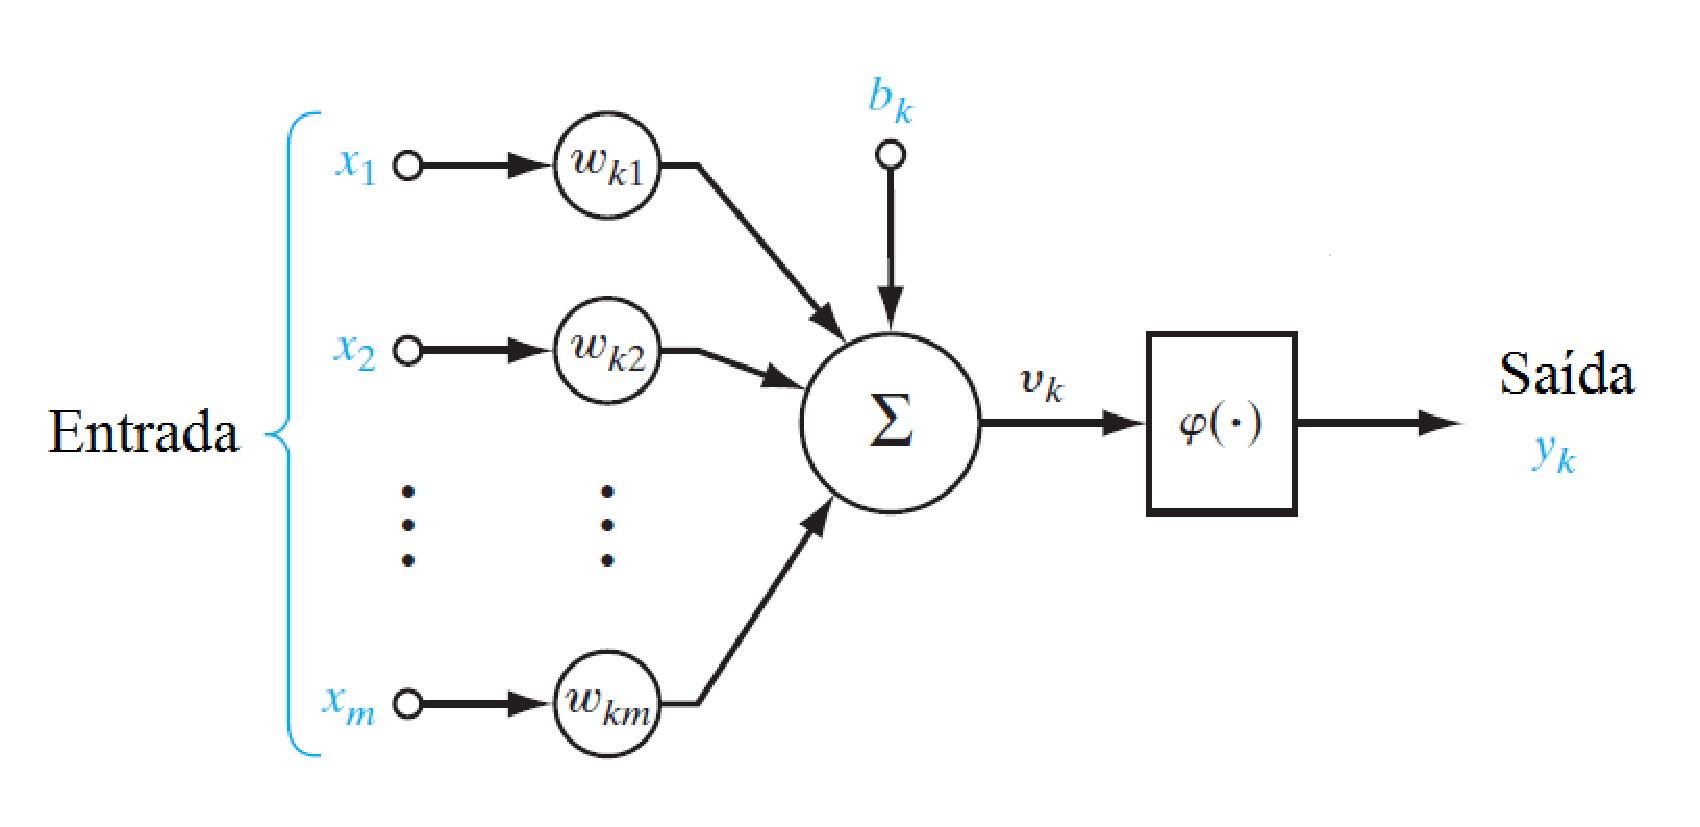
\includegraphics[width=0.7\textwidth]{./fig/neuronio}
 \caption{Modelo de um neurônio artificial \cite{santamaria2018}.}
 \label{fig:neuronio}
\end{figure}

Os pesos podem assumir valores positivos ou negativos, sendo seus valores ajustados em um processo de otimização, codificando o conhecimento adquirido pela rede. O modelo também inclui um \textit{bias} $b_{k}$, utilizado para aumentar o grau de liberdade dos ajustes dos pesos, permitindo uma melhor adaptação, por parte da rede neural, ao conhecimento a ela fornecido.

As funções de ativação introduzem um componente não linear às redes neurais, fazendo com que aprendam mais do que relações lineares entre as variáveis dependentes e independentes. Elas basicamente decidem se um neurônio deve ser ativado ou não, ou seja, se a informação que o neurônio está recebendo é relevante ou deve ser ignorada \cite{deeplearningb}.  Alguns exemplos de funções de ativação são observados na Figura \ref{fig:activacao}.

\begin{figure}[ht]
  \centering
  \subfigure[Degrau]
   {
    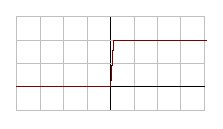
\includegraphics[width=0.3\textwidth]{./fig/Activation_binary_step}
    \label{subfig:bi}
   } 
  \subfigure[Sigmoidal]
   {
    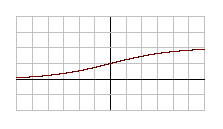
\includegraphics[width=0.3\textwidth]{./fig/Activation_logistic}
    \label{subfig:sig}
   }
   \subfigure[Gaussiana]
   {
    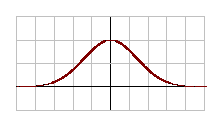
\includegraphics[width=0.3\textwidth]{./fig/Activation_gaussian}
    \label{subfig:gauss}
   }
   \caption{Exemplos de funções de ativação.}
  \label{fig:activacao}
\end{figure}

Os neurônios costumam ser divididos em camadas, onde existe uma camada de neurônios de entrada, podendo ser conectada a uma ou diversas camadas intermediárias que, por sua vez, se conectam aos neurônios da camada de saída, como mostra a Figura \ref{fig:redeneural}. A camada de entrada é responsável pelo recebimento dos dados a serem analisados, assim como a correspondente associação com os pesos de entrada. As camadas intermediárias tem por finalidade extrair as informações associadas ao sistema inferido, sendo também responsável pela maior parte do processamento destes dados. Já a camada de saída agrega as informações das camadas anteriores e ativa uma resposta adequada.

\begin{figure}[H]
 \centering
  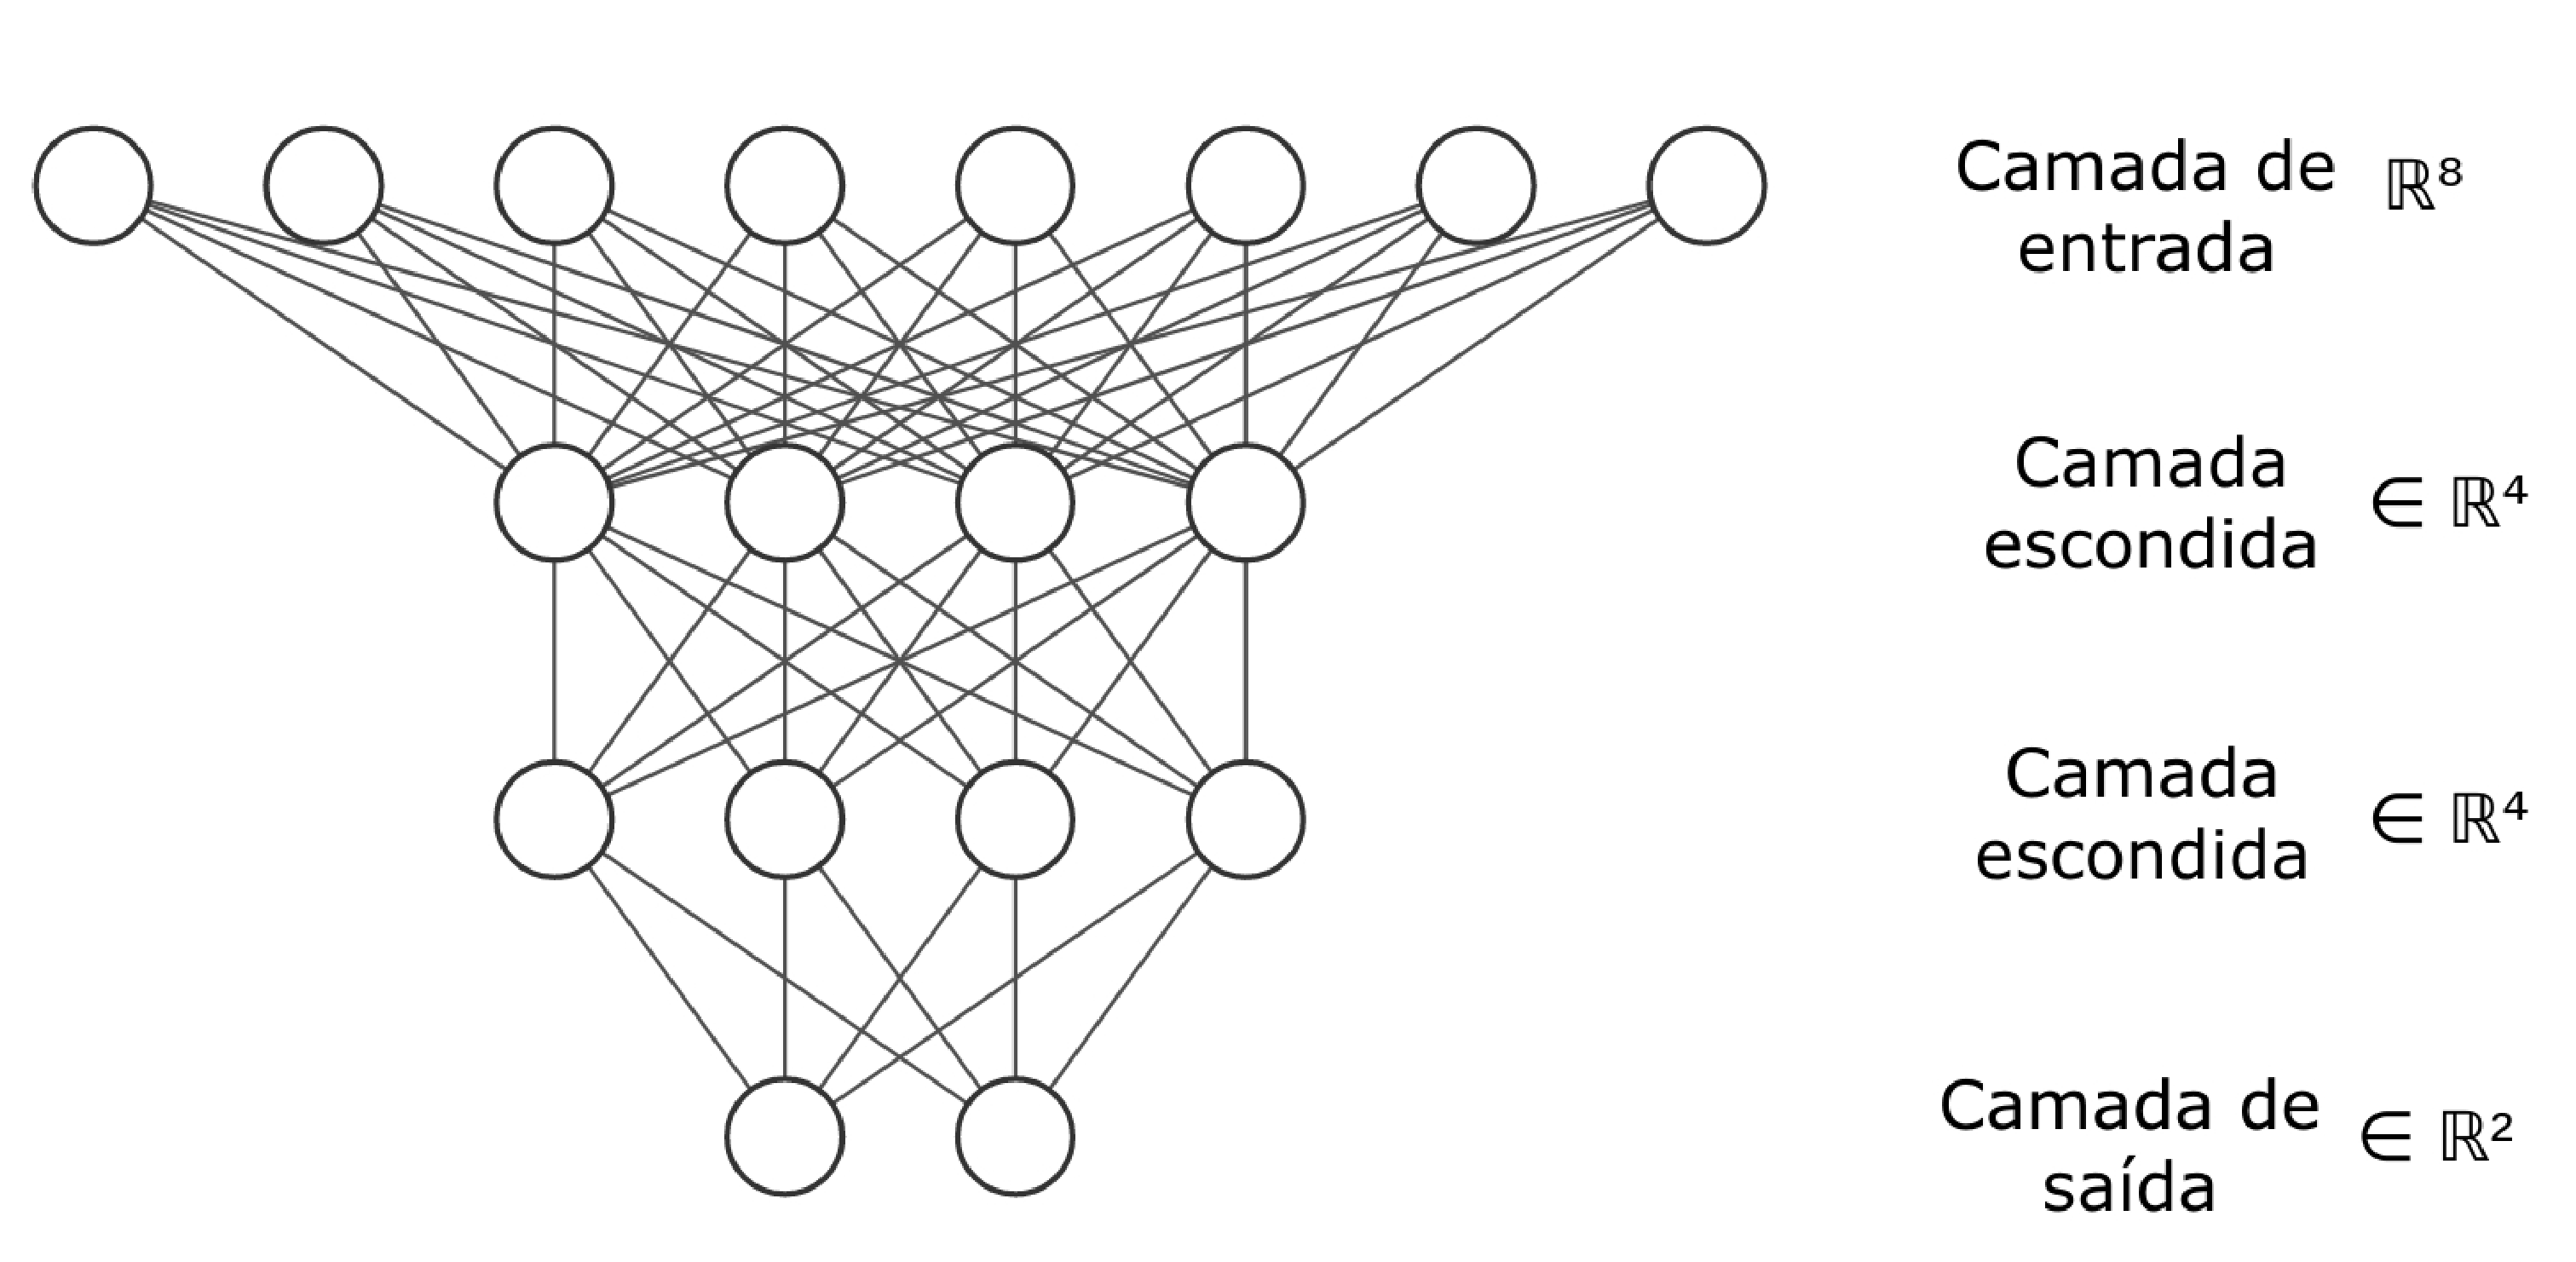
\includegraphics[width=0.8\textwidth]{./fig/nn}
 \caption{Rede neural com duas camadas intermediárias.}
 \label{fig:redeneural}
\end{figure}

Redes neurais com muitas camadas intermediárias são ditas redes neurais profundas. Nessas redes, os dados são submetidos a um processo de várias etapas de reconhecimento de padrões, cada camada sendo é responsável por reconhecer um conjunto de características diferente. Quanto mais profundo na rede, mais complexas serão as características reconhecidas, uma vez os dados são agregados e recombinados da camada anterior. 

As conexões de uma RNA define como os neurônios são conectados entre si, podendo ser classificadas em redes diretas (\textit{feedforward}) ou redes recorrentes. Nas redes diretas, as informações fluem da camada de entrada para os neurônios da camada de saída. Já as conexões das redes recorrentes permitem que um neurônio receba a saída de um neurônio da mesma camada, de uma camada posterior, ou até mesmo a sua própria saída. Os sistemas baseados em RNAs, dependem fortemente da topologia destas redes (tamanho, estrutura, conexões), assim como de seus parâmetros. Como resultado, a determinação da arquitetura da rede afeta muito o seu desempenho, isto é, velocidade de aprendizado, exatidão do aprendizado, tolerância a ruídos e capacidade de generalização.

Dentre as topologias existentes, têm-se as Redes Neurais Convolucionais (CNN, do inglês \textit{Convolutional Neural Network}), que utilizam uma arquitetura especial que é particularmente bem adaptada para classificar imagens \cite{Krizhevsky12}. O ponto central de uma CNN são as camadas convolucionais, que dão o nome da rede. Uma convolução, nesse contexto, é uma operação linear que envolve a multiplicação de um conjunto de pesos ao conjunto de entrada. Como a entrada dessa rede é de natureza bi-dimensional, a multiplicação é realizada entre a entrada e vetores bi-dimensionais de pesos, chamados de filtros. Cada um dos filtros é responsável por aprender uma determinada característica nos dados de entrada.

Um método comum para o treinamento de uma rede neural é o algoritmo de \textit{backpropagation}  \cite{rumelhart86}. Em um processo de otimização, a rede neural transmite o sinal dos dados de entrada até a camada de saída, através de seus parâmetros. O gradiente de uma função de custo é então retro-propagado pela rede para que seus pesos possam ser alterados, visando minimizar essa função. 

Nas últimas décadas, com a crescente complexidade dos problemas a serem tratados computacionalmente e do volume de dados gerados por diferentes setores, o uso de RNA se tornou cada vez mais comum. As redes neurais profundas são responsáveis por avanços recentes em uma grande variedade de tarefas difíceis de se resolver utilizando programação baseada em regras comuns, como, por exemplo, áreas de visão computacional \cite{Krizhevsky12}, de reconhecimento de fala \cite{NassifSAAS19} e do processamento de linguagem natural \cite{otter2018}.

%% - - - - - - - - - - - - - - - - - - - - - - - - - - - - - - - - - - -
\section{Aprendizado de Máquina}

% Um algoritmo é uma sequência de ações/etapas que levam à uma solução de um problema. Na computação, portanto, um algoritmo é uma ferramenta para solucionar problemas computacionais descritos e especificados, dado um conjunto de entrada. Entretanto, alguns problemas são difíceis de se estabelecer uma sequência de passos finitos para ser realizado, ou obter uma sequência de passos que irão gerar um conjunto de saída em um tempo não exorbitante. Um mundo onde tem-se uma carga de informação impossível de ser acompanhada por qualquer ser humano, onde há toneladas de dados e informações a serem analisadas, a Inteligência Artificial (IA) entra como agente capaz de automatizar a aprendizagem repetitiva por meio da análise de dados.

O aprendizado de máquina pode ser definido como a área da Inteligência Artificial relacionada à busca de um conjunto de regras/padrões que permitem que as máquinas tomem decisões baseadas em um grande conjunto de dados sem serem especificamente programadas para essa tomada de decisões \cite{Samuel59}. Em outras palavras, o aprendizado de máquina é o processo de encontrar um modelo ou hipótese que aproxima uma função alvo usando um conjunto de dados de treinamento. Depois que a máquina é treinada, a hipótese final deve satisfazer os dados de treinamento bem como dados não vistos anteriormente.

Tradicionalmente, essa área é dividida em três diferentes categorias, baseadas na natureza do tipo de aprendizagem: aprendizado supervisionado, aprendizado não supervisionado, e aprendizado por reforço. Além disso, há abordagens de otimização estocástica, como computação evolutiva, para aprendizado \cite{Salimans2017}. Todas essas abordagens são candidatas viáveis de treinamento para jogos eletrônicos \cite{justesen2018}.

O Aprendizado Supervisionado consiste na tarefa de inferir uma função a partir de dados de treinamento rotulados (par composto por um objeto de entrada e um valor de saída desejado), com a finalidade de prever rótulos desconhecidos em um conjunto de teste, podendo o rótulo ser um conjunto finito ou um valor real. Em contra-partida, no aprendizado não supervisionado não há nenhum tipo de orientação para verificar se a predição está correta e o objetivo passa a ser encontrar padrões nos dados. Já no aprendizado por reforço, um agente interage com um ambiente e seu o objetivo é aprender um comportamento através dessa interação, visando maximizar um valor de retorno, chamado de recompensa.

%% - - - - - - - - - - - - - - - - - - - - - - - - - - - - - - - - - - -
\section{Aprendizado por Reforço}

Aprendizado por reforço é a área de aprendizado de máquina cujo objetivo reside em criar agentes artificiais que possuem a capacidade de alcançar um nível equivalente de performance e generalização dos seres humanos \cite{deepmind}. 

O aprendizado se dá pela interação do agente com o ambiente em que ele se encontra. Essa interação é representada pela escolha de ações a serem executadas no ambiente, que levam a mudanças de estados. Dessa interação, o agente obtém sinais de retorno, que irão categorizar se a ação tomada foi uma boa ou má escolha. Os sinais de retorno, também chamados de recompensa, podem ocorrer com frequência, como a alteração na pontuação dentro de um jogo, ou com pouca frequência, como se um agente ganhou ou perdeu um jogo. Todo esse processo de escolhas de ações se dá por tentativa e erro do agente, tornando esse modelo de aprendizado o mais próximo do processo de aprendizado dos seres humanos e animais.

Um Processo de Decisão de Markov (MDP, do inglês \textit{Markov Decision Process}) fornece uma estrutura matemática para modelagem de tomada de decisão em situações onde os resultados são em parte aleatórios e em parte sob o controle de um tomador de decisão \cite{sutton-barto98}. Se um ambiente pode ser descrito como um MDP, então o agente pode construir uma árvore de probabilidade de estados futuros e suas recompensas, que poderá ser utilizada para calcular o valor do estado atual \cite{Lapan2018}. A figura \ref{fig:rl} mostra a interação agente-ambiente em um MDP.

\begin{figure}[ht]
 \centering
  \includegraphics[width=0.70\textwidth]{./fig/RL}
 \caption{Interação agente-ambiente em um Processo de Decisão de Markov \cite{sutton-barto98}.}
 \label{fig:rl}
\end{figure}

Temos que um MDP consiste de um conjunto finito de estados $S$, um conjunto de possíveis ações $A(s)$ para cada estado, um valor de retorno $R$ para cada estado, e um modelo de transição $P(s'|s,a)$. Para cada episódio no tempo $t$, o retorno é definida por:

\begin{equation}
R_t = r_{t+1} + \gamma r_{t+2} + ... =  \sum^{\infty}_{k=0}\gamma^k r_{t+k+1}
\end{equation}

O retorno é calculado como uma soma de recompensas subsequentes. Um fator de desconto $\gamma$ é utilizado para recompensas mais distantes do ponto de início $t$, definindo a visibilidade do agente. Entretanto, esse valor de retorno a longo prazo não é muito útil na prática: o agente pode tomar diferentes ações resultando em diferentes caminhos para um mesmo estado \cite{Lapan2018}. Para isso, temos uma função de retorno mais útil, a função de valor (Equação \ref{eqn:value}), que consiste na predição do valor de retorno a longo prazo.

\begin{equation}
\label{eqn:value}
V(s) = \E \left[\sum^{T}_{t=1}\gamma^{t-1}r_{i}\right] \forall s \in S
\end{equation}

A função de valor representa o quão bom um estado é com base em sua recompensa. O objetivo do agente é maximizar esse valor. Entretanto, para alcançar bons estados é necessário escolher ações que levam para esses estados. Para isso, temos a política, que define o comportamento do agente, ou seja, uma política diz para o agente o que fazer em uma determinada situação \cite{Lapan2018}. Formalmente, política é definida como uma distribuição de probabilidades sobre ações $a$ para cada possível estado $s$ em um dado tempo $t$ (Equação \ref{eqn:estocastico}), ou como um simples mapeamento de estados para ações (Equação \ref{eqn:determistico}).

\begin{equation}
\label{eqn:estocastico}
\pi(a|s) = P(A_t = a|S_t = s)
\end{equation}

\begin{equation}
\label{eqn:determistico}
\pi(s) = a
\end{equation}

Há algumas abordagens para resolver um problema de aprendizado por reforço. Dentre elas temos os métodos baseados em valor e métodos baseados em política. Métodos baseados em valor focam em encontrar ou aproximar a função de valor ideal que maximizam a recompensa, enquanto sua política é mantida de tal forma a escolher o par de ação-estado que obtém a maior recompensa. Métodos baseados em política, tentam encontrar a política ideal diretamente, sem consultar a função valor, buscando também maximizar a recompensa. Ambos os métodos baseados em valor e em política são ditos livre de modelo, ou seja, ignoramos o modelo e dependemos apenas da amostragem e simulação para estimar as recompensas, para que não seja preciso conhecer o funcionamento interno do sistema. Já métodos baseados em modelo, se podemos definir uma função de recompensa, podemos calcular as ações ideais usando o modelo diretamente. 

Mesmo não precisando levar em consideração a política durante o aprendizado, todo algoritmo de aprendizado por reforço deve seguir alguma política para decidir quais ações executar em cada estado. Algoritmos que levam em consideração a política que gerou decisões passadas de ação-estado são chamados de algoritmos \textit{on-policy}, enquanto aqueles que a ignoram são conhecidos \textit{off-policy}. Algoritmos \textit{off-policy} geralmente empregam uma política de comportamento separada, independente da política que está sendo aprimorada; a política de comportamento é usada para simular trajetórias. Um algoritmo \textit{off-policy} bem conhecido é o \textit{Q-Learning} \cite{Watkins92}. Sua regra de atualização usa a ação que produzirá o \textit{Q-Value} mais alto, enquanto que a verdadeira política usada pode restringir essa ação ou escolher outra. O \textit{Q-value} é uma medida da recompensa geral esperada, assumindo que o agente esteja no estado $s$ e executa uma ação $a$, e continua a jogar até o final do episódio, seguindo alguma política $\pi$. A variação \textit{on-policy} do \textit{Q-learning} é o SARSA \cite{rummery94}, onde a regra de atualização usa a ação escolhida pela política seguida.


%% - - - - - - - - - - - - - - - - - - - - - - - - - - - - - - - - - - -
\section{Métodos de Gradiente de Política}

Em métodos baseados em política e, em especial, métodos de gradiente de política, o objetivo é aprender uma política que consegue selecionar ações sem consultar a função de valor diretamente. Nesse método a política pode ser tanto determinística quanto estocástica, além de ser possível de se trabalhar com um espaço de ações contínua \cite{Lapan2018}. Quando o agente obtém uma observação e precisa tomar uma ação precisamos da política, ou seja, é da política que precisamos ao resolver um problema de aprendizado de reforço.

Como qualquer configuração de aprendizado de máquina, pode-se definir um conjunto de parâmetros $\theta$ (como por exemplo, os pesos e \textit{bias} das redes neurais) para parametrizar uma política - $\pi_{\theta}$. O objetivo é buscar os parâmetros $\theta$ que maximizam a recompensa obtida, portanto, uma abordagem para resolver esse problema é o método do gradiente (Equação \ref{eqn:objpg}). No gradiente, continuamente percorremos os parâmetros usando a regra de atualização da Equação \ref{eqn:pgrad}. A recompensa $R_t$ guia a atualização, enquanto que a taxa de aprendizado $\alpha$ define a magnitude do ajuste feito nas atualizações \cite{sutton-barto98}.

\begin{equation}
\label{eqn:objpg}
\nabla_{\theta}J(\theta) = \E_{t\sim\pi_{\theta}} \left[\sum^{T}_{t=0}\nabla_{\theta}log\pi_{\theta}(a_t|s_t)R_t\right]
\end{equation}

\begin{equation}
\label{eqn:pgrad}
\theta_{t+1} = \theta_{t} + \alpha \nabla_{\theta} J(\pi_{\theta_k})
\end{equation}

A Equação \ref{eqn:objpg} mede a probabilidade da trajetória sob a política atual. O uso da função de recompensa aumenta a probabilidade de uma política se a trajetória resultar em uma alta recompensa positiva. Por outro lado, diminui a probabilidade de uma política se resultar em uma alta recompensa negativa. Entretanto, a função de recompensa pode impedir a exploração de políticas que poderiam levar a uma recompensa maior, uma vez que um único caminho que leva o agente obter recompensas positivas seria reforçado sempre. O método de gradiente é um método de derivada de primeira ordem, não sendo muito confiável se a função de recompensa tiver uma curvatura muito íngreme \cite{jonathanHuiRL}. Para resolver isso, é utilizado a função de vantagem (Equação \ref{eqn:advantage}) em vez da recompensa esperada, por reduzir a variação da estimativa \cite{jonathanHuiPPO}.

\begin{equation}
\label{eqn:advantage}
A_{t}^{(n)}(s,a) = r_{t} + \gamma V(s_{t+1}) + ... + \gamma^n V(s_{t+n}) - V(s_{t})
\end{equation}

A função de vantagem é uma medida de quanto uma determinada ação é uma decisão boa ou ruim, dado um determinado estado. Em outras palavras, a função informa sobre a recompensa extra que poderia ser obtida pelo agente, executando essa ação específica. Se $A_{t}(s,a) > 0$ o gradiente é empurrado nessa direção. Se $A_{t}(s,a) < 0$, ou seja, a ação escolhida é pior que o valor médio desse estado, o gradiente é empurrado na direção oposta.

A Equação \ref{eqn:advantage} assume a forma de estimadores de diferença temporal, onde primeiro é estimado a soma das recompensas com desconto e então é descontado a estimativa da função de valor. Para $A_{t}^{(n)}$ com valores baixos de $n$ a estimativa terá baixa variação, mas alto viés, enquanto para valores altos de $n$ a estimativa terá viés baixo, mas alta variação \cite{seita}. Dado esse dilema de viés e variância, foi proposto uma abordagem mais geral para calcular a vantagem, a Estimativa de Vantagem Generalizada (GAE, do inglês \textit{Generalized Advantage Estimation}) \cite{Schulman16}.

\begin{equation}
\label{eqn:temporaldiscount}
\delta^{V}_{t} = r_{t} + \gamma V(s_{t+1}) - V(s_{t})
\end{equation}

\begin{equation}
\label{eqn:gae}
A_{t}^{GAE(\gamma, \lambda)} = \sum_{l=0}^{\infty} \left(\gamma\lambda\right)^{l}\delta^{V}_{t}
\end{equation}

A Equação \ref{eqn:gae} é um estimador de vantagem com dois parâmetros separados $\gamma$ e $\lambda$, os quais contribuem para o balanceamento entre a variação e o viés. No entanto, ambos os parâmetros servem a propósitos diferentes e funcionam melhor com diferentes faixas de valores \cite{Schulman16}. O fator $\gamma$ ainda definirá o desconto de recompensas futuras, enquanto que o fator $\lambda$ é responsável pelo balanceamento entre o viés e a variação.


%% - - - - - - - - - - - - - - - - - - - - - - - - - - - - - - - - - - -
\section{\textit{Proximal Policy Optimization}}
\label{section:ppoalg}

Alguns problemas dos métodos de gradiente de política aparecem da taxa de aprendizado: se for muito pequena o processo de treinamento será muito lento, porém se for muito alta terá muita variabilidade no treinamento. A ideia central do algoritmo \textit{Proximal Policy Optimization} (PPO) \cite{Schulman17} é evitar grandes atualizações de políticas. A taxa de aprendizado restringe as atualizações relacionadas aos parâmetros, enquanto que o PPO leva em consideração as probabilidades das ações, utilizando uma proporção que indica a diferença entre uma nova política e uma política antiga (Equação \ref{eqn:ratio}). Como as probabilidades das ações que definem o comportamento da política, estabilizá-los entre as atualizações garante uma maior estabilidade \cite{Schulman15}. 

\begin{equation}
\label{eqn:ratio}
r_{t} = \frac{\pi_{\theta}(a_{t}|s_{t})} {\pi_{\theta_{old}}(a_{t}|s_{t})} 
\end{equation}

Se $r_{t}(\theta) > 1$ então a ação é mais provável na política atual do que na política antiga, enquanto que se $r_{t}(\theta)$ está entre 0 e 1 a ação é menos provável na nova política do que na antiga. Entretanto, a ausência de uma restrição pode levar a grandes atualizações \cite{Schulman17}. O que o PPO faz é tentar garantir pequenas alterações restringindo a razão de probabilidade das políticas, penalizando grandes passos que levam a políticas muito diferentes. Dessa maneira teremos duas proporções, uma sem restrição e uma restringida a um intervalo (entre $[1-\epsilon, 1+\epsilon]$, onde $\epsilon$ é um hiper-parâmetro). Então, pega-se o mínimo entre esses valores, sendo o objetivo final um limite inferior para a atualização da política, evitando grandes atualizações. A nova função objetivo fica definida como:

\begin{equation}
\label{eqn:clip}
L^{CLIP}(\theta) = \E_{t} \left[min(r_{t}(\theta)A_{ t}, clip(r_{t}(\theta), 1-\epsilon, 1+\epsilon)A_{t}\right]
\end{equation}

\begin{figure}[ht]
 \centering
  \includegraphics[width=0.80\textwidth]{./fig/clip}
  \captionsetup{width=1\textwidth}
 \caption[Gráficos da função $L^{CLIP}$.]
 {Gráficos da função $L^{CLIP}$. Valores em função da razão de probabilidade $r$, para vantagens positivas (esquerda) e vantagens negativas (direita) \cite{Schulman17}.}
 \label{fig:ppoclip}
\end{figure}

A nova função objetivo (Equação \ref{eqn:clip}) reduz a vantagem estimada se a nova política estiver longe da antiga. Se uma ação é muito mais provável sob a nova política do que a antiga, não queremos exagerar na atualização da ação, então restringimos a função objetivo. Se a nova política for muito menos provável do que a antiga, novamente deve-se impedir atualizações exageradas.

O PPO tenta delimitar uma pequena região para atualizações, mas trata o problema como um método iterativo de otimização, onde é possível utilizar gradiente ascendente. O Algoritmo \ref{alg:ppoclip} representa o funcionamento do PPO com objetivo limitado \cite{Achiam}. Primeiro, avalia-se a política sobre um conjunto de dados, e então realiza-se melhorias aplicando atualizações de otimização da Equação \ref{eqn:clip}. Durante o período de avaliação, a função de vantagem $A^\pi$ da política atual $\pi$ será estimada. Em seguida, é possível modificar a política atual executando atualizações com base na função de vantagem. Depois de gerar essa nova política, voltamos à avaliação. Esse ciclo ocorre até encontrarmos a função de vantagem e política ideais.


\medskip
\begin{center}
\begin{minipage}{0.92\textwidth}
\begin{algorithm2e}[H]
 \DontPrintSemicolon
 \Entrada{parâmetros da política inicial $\theta_0$, limiar de corte $\epsilon$}
 \Para{$k= 0, 1, 2, ...$}
   {Colete um conjunto de trajetórias $D_k$ com política $\pi_k = \pi(\theta_{k})$ \\
    Estime a função de vantagem $A_{t}^{GAE(\gamma, \lambda)}$ \\
    Calcule a atualização da política \\
    \hspace{3cm}$\theta_{k+1} = arg \max_{\theta}L^{CLIP}_{\theta_k}(\theta)$ \\
    executando N etapas do gradiente ascendente, onde \\
    \hspace{2cm}$L^{CLIP}_{\theta_k}(\theta) = \E_{t} \left[min(r_{t}(\theta)A_{ t}, clip(r_{t}(\theta), 1-\epsilon, 1+\epsilon)A_{t}\right]$ 
   }
\caption{\textit{Proximal Policy Optimization} com objetivo limitado \label{alg:ppoclip}}
\end{algorithm2e}
\end{minipage}
\end{center}

% \input{./tex/cap_III}
\chapter{Metodologia}
\label{cap:metodologia}

Este trabalho tem como proposta utilizar os conceitos antecedentes e as ferramentas apresentadas na seção seguinte para construção e treinamento de um agente de aprendizado por reforço, a fim de que se possa analisar sua capacidade de abstrair informações, generalizando o conhecimento obtido de uma fase de treinamento e sendo capaz de atuar em um ambiente com elementos não vistos anteriormente. Para isso, neste Capítulo será apresentada uma descrição do projeto realizado, fazendo uso das técnicas descritas no Capítulo \ref{cap:fundamento} aplicadas ao ambiente simulado \textit{General Video Game Artificial Intelligence}, para a análise da capacidade de generalização do algoritmo \textit{Proximal Policy Optimization}. Ao final, são descritos os experimentos realizados para validação da proposta.

% - - - - - - - - - - - - - - - - - - - - - - - - - - - - - - - - - - -
\section{\textit{General Video Game Artificial Intelligence}}

Recentemente, pesquisadores começaram a explorar sistematicamente a generalização em aprendizado por reforço, desenvolvendo novos ambientes simulados que permitem criar uma distribuição de Processo de Decisão de Markov e dividir instâncias únicas de treinamento e teste, buscando fugir das limitações de ambientes baseados em jogos existentes. Tais limitações são decorrentes da ausência de disponibilidade de avaliação do agente em jogos nos quais não foi treinado, limitações essas que impedem a avaliação do aspecto de generalidade do algoritmo utilizado. Com base nisso foi desenvolvida uma \textit{framework} e competição de mesmo nome: o \textit{General Video Game Artificial Intelligence} (GVGAI) \cite{torrado18, perez18}. 

A \textit{framework} trabalha com a ideia de medir o desempenho do agente em um grande número de ambientes, que poderiam ser jogos amostrados de um espaço de jogo \cite{schaul11}. Os ambientes, nesse caso, são definidos por meio de uma Linguagem de Descrição de \textit{Video Games} (VGDL, do inglês \textit{Video Game Description Language}) \cite{Schaul13}, que permite facilmente customizar jogos e níveis, possibilitando a criação de variantes dos jogos em pouco tempo \cite{gvgaibook2019}. Na competição de aprendizado do GVGAI, os competidores possuem a sua disposição um conjunto de três fases de um jogo a ser utilizado no treinamento de um agente inteligente. A validação do agente é realizada sobre outras duas fases do mesmo jogo, e os resultados obtidos nesses níveis de validação são os utilizados na competição para classificar as entradas.

A estrutura do GVGAI é conectada através da interface do Gym (GVGAI\_GYM\footnote{\url{https://github.com/rubenrtorrado/GVGAI\_GYM}}), que consiste em um conjunto de ferramentas que permite desenvolver e comparar algoritmos de aprendizado por reforço \cite{gymOpenai}. Essa ferramenta permite flexibilidade, visto que não faz suposições sobre a estrutura do agente. Os ambientes providos retornam os valores de observação e recompensa ao informar a ação selecionada, além de informar também sobre o término de um episódio, seja porque o agente cumpriu o seu objetivo ou está incapacitado de cumpri-lo. Na Figura \ref{fig:gym} está ilustrado o fluxo de funcionamento da interface GYM em relação ao ambiente e ao agente.

\begin{figure}[ht]
 \centering
  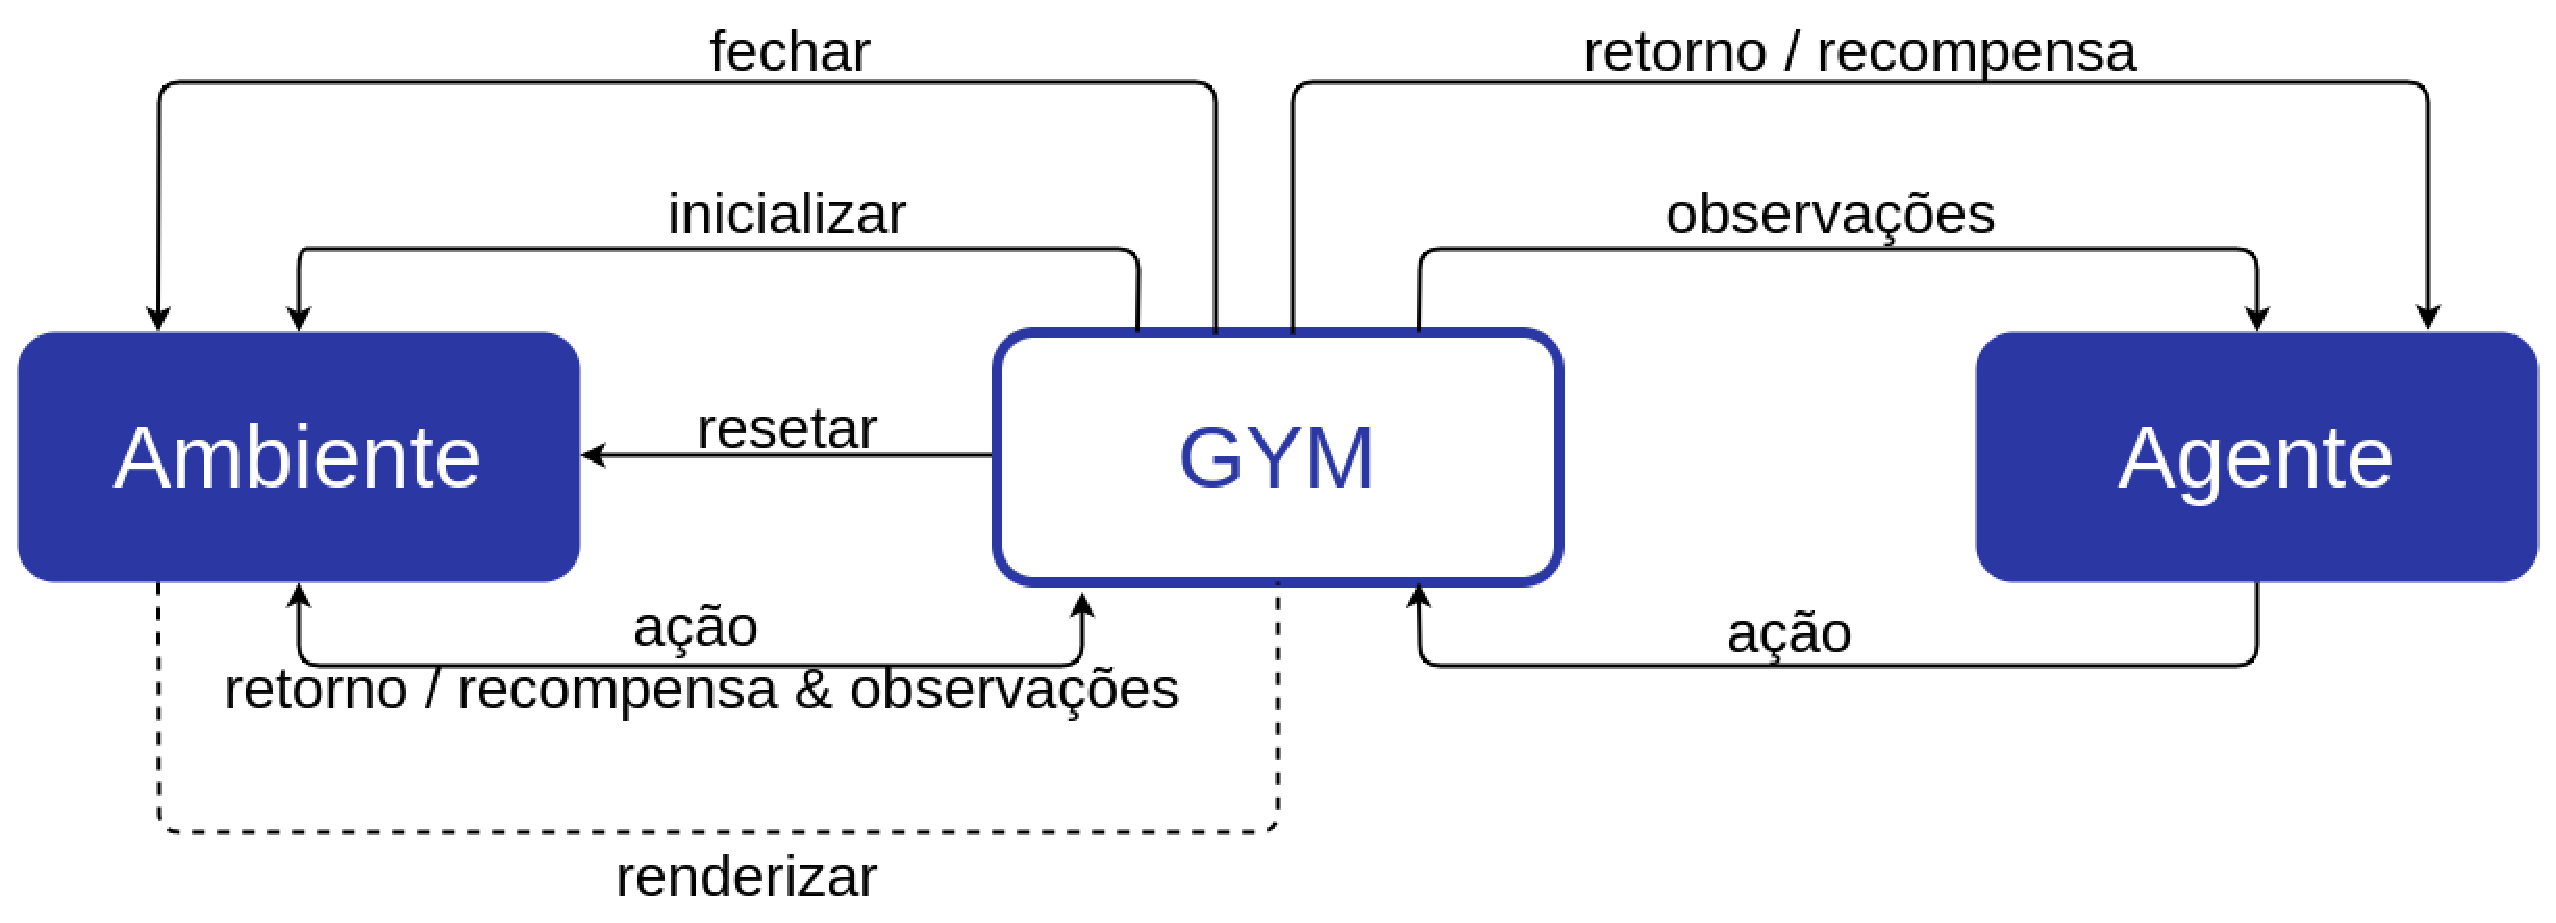
\includegraphics[width=0.9\textwidth]{./fig/gym}
 \caption{Fluxo de funcionamento da ferramenta GYM.}
 \label{fig:gym}
\end{figure}

Os jogos disponíveis no GVGAI\_GYM são jogos bidimensionais do tipo arcade. Jogos de arcade, geralmente, possuem níveis de curta duração, controles simples e uma dificuldade crescente, exigindo bons reflexos e pensamento estratégico dos seus jogadores. A Figura \ref{fig:jogosgvgai}\subref{subfig:super} é referente ao jogo \textit{Superman} e a \ref{fig:jogosgvgai}\subref{subfig:super} ao jogo \textit{Wait For Breakfast}, ambos disponíveis no GVGAI\_GYM.

\begin{figure}[ht]
  \centering
  \subfigure[\textit{Superman}]
  {
    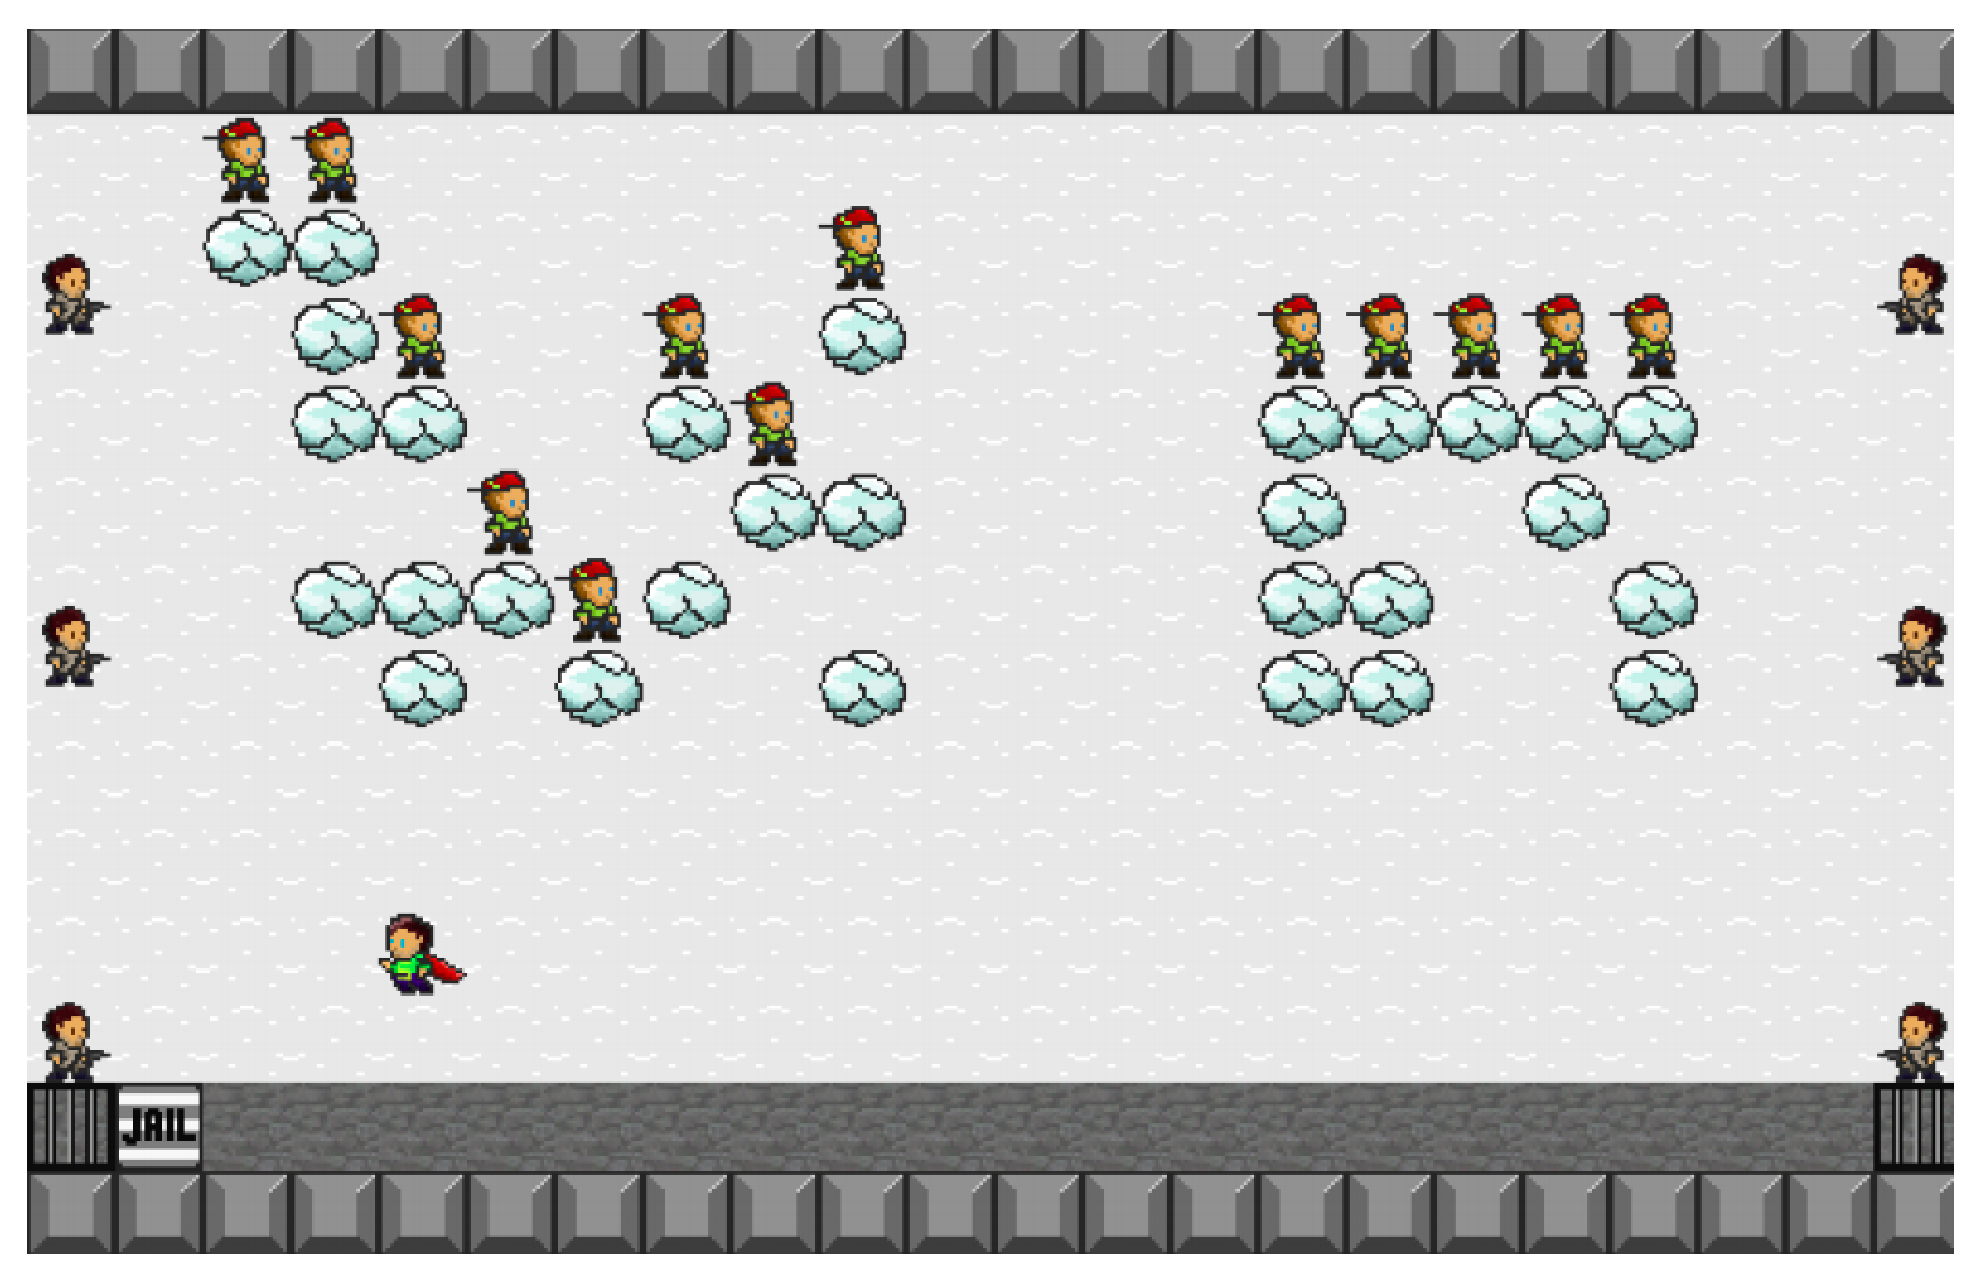
\includegraphics[width=0.42\textwidth]{./fig/superman}
    \label{subfig:super}
  } \qquad
  \subfigure[\textit{Wait For Breakfast}]
  {
    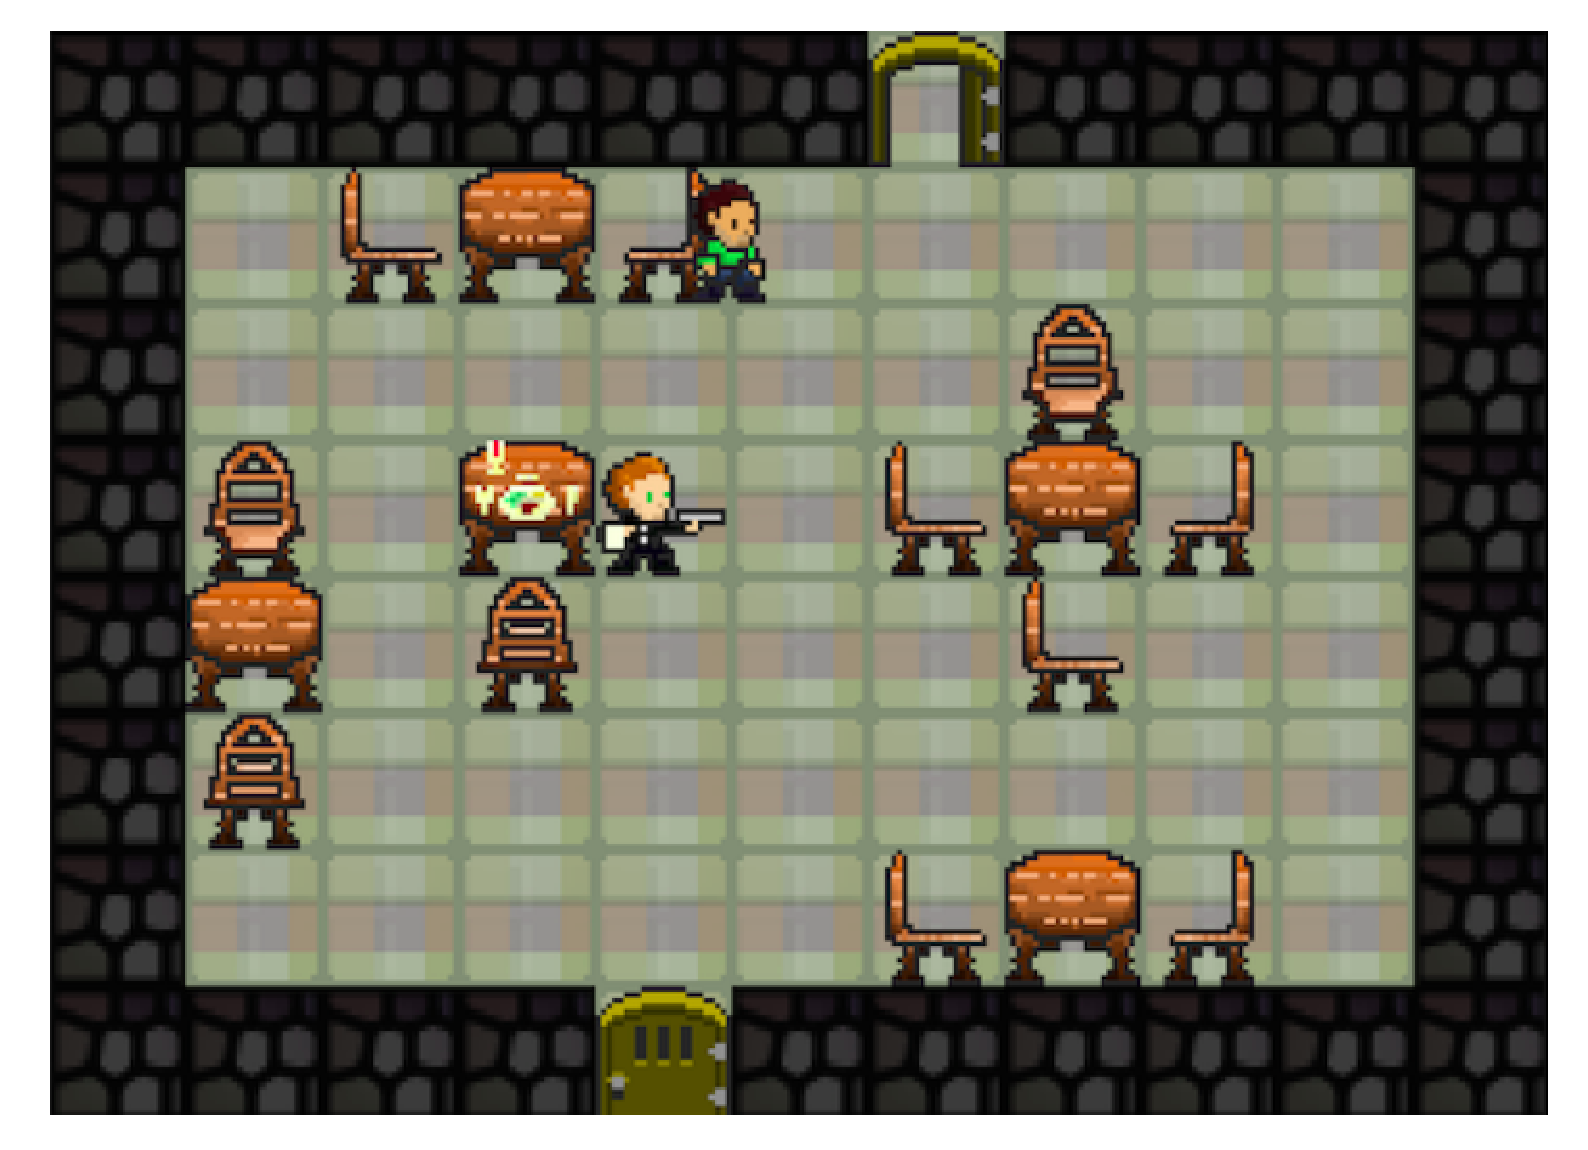
\includegraphics[width=0.38\textwidth]{./fig/waitForBreakfast}
    \label{subfig:wait}
  }
  \caption{Exemplos de jogos disponíveis no GVGAI\_GYM \cite{torrado18}.}
  \label{fig:jogosgvgai}
\end{figure}

% - - - - - - - - - - - - - - - - - - - - - - - - - - - - - - - - - - -

Para os testes da proposta desenvolvida neste trabalho, serão utilizados os jogos \textit{Aliens}, \textit{Boulder Dash} e \textit{Missile Commands}. No primeiro jogo, \textit{Aliens} (Figura \ref{fig:aliens}), as principais tarefas são evitar projéteis inimigos recebidos e disparar no momento certo para atingir o inimigo. Todos os personagens não jogáveis e projéteis se comportam de maneira determinística (projéteis inimigos são disparados estocasticamente, mas leva algum tempo para alcançar o jogador). 

Já no jogo \textit{Boulder Dash} (Figura \ref{fig:boulderdash}), o jogador deve explorar cavernas, coletando diamantes e chegando a uma saída dentro de um prazo, evitando criaturas perigosas e obstáculos. \textit{Boulder Dash} exige que seu jogador possua reações rápidas para evitar quedas de pedras, e planejamento estratégico a longo prazo  para escavar terra e coletar diamantes não ficando preso entre as pedras. 

Por fim, no jogo \textit{Missile Command} (Figura \ref{fig:missilecommand}), cidades estão sendo atacadas por mísseis e o jogador deve destruí-los utilizando os canhões disponíveis. Os mísseis disparados pelo jogador explodem ao atingir a mira, deixando uma bola de fogo que persiste por alguns segundos e destruindo quaisquer mísseis inimigos que entrem nela. Um recompensa positiva é recebida para cada míssil inimigo destruído, e uma recompensa negativa para cada canhão destruído.

\begin{figure}[h]
  \centering
  \subfigure
  {
    \includegraphics[width=0.39\textwidth]{./fig/gvgai-aliens-lvl0-v0}
    \label{subfig:aliens1}
  } 
  \subfigure
  {
    \includegraphics[width=0.39\textwidth]{./fig/gvgai-aliens-lvl4-v0}
    \label{subfig:aliens3}
  }
  \caption{Captura de tela do jogo \textit{Aliens}.}
  \label{fig:aliens}
\end{figure}

\begin{figure}[h]
  \centering
  \subfigure
  {
    \includegraphics[width=0.39\textwidth]{./fig/gvgai-boulderdash-lvl0-v0}
    \label{subfig:boulderdash1}
  } 
  \subfigure
  {
    \includegraphics[width=0.39\textwidth]{./fig/gvgai-boulderdash-lvl2-v0}
    \label{subfig:boulderdash3}
  }
  \caption{Captura de tela do jogo \textit{Boulder Dash}.}
  \label{fig:boulderdash}
\end{figure}


\begin{figure}[h]
  \centering
  \subfigure
  {
    \includegraphics[width=0.39\textwidth]{./fig/gvgai-missilecommand-lvl0-v0}
    \label{subfig:missilecommand1}
  } 
  \subfigure
  {
    \includegraphics[width=0.39\textwidth]{./fig/gvgai-missilecommand-lvl2-v0}
    \label{subfig:missilecommand3}
  }
  \caption{Captura de tela do jogo \textit{Missile Command}.}
  \label{fig:missilecommand}
\end{figure}

% - - - - - - - - - - - - - - - - - - - - - - - - - - - - - - - - - - -
\section{Algoritmo de Treinamento}

A arquitetura do agente de aprendizado por reforço consiste em duas partes: o algoritmo \textit{Proximal Policy Optimization} e o ambiente de simulação fornecido pelo GVGAI\_GYM. Os ambientes do GVGAI\_GYM se diferenciam em dois aspectos importantes para o agente: o tamanho do espaço de ações disponíveis e o tamanho da imagem do jogo. As imagens são referentes aos estados observáveis do jogo que são passadas para o agente. Para obter dados mais relevantes das observações e tornar o algoritmo mais computacionalmente eficiente, é realizado um pré-processamento nas imagens de entrada. O processo consiste em eliminar as cores presentes na imagem, transformando-a em uma escala de cinza, e redimensionando o tamanho das imagens para o tamanho padrão de $84x84$ \textit{pixels}. A Figura \ref{fig:jogosanalisepp} apresenta a saída do pré-processamento feito sobre uma imagem do jogo. Por fim, é combinado várias imagens em uma única entrada, fazendo com que o modelo escolha ações com base em uma série de quadros em vez de apenas um único quadro. Isso permite ao modelo discernir coisas como a direção do personagem ou sua velocidade.

\begin{figure}[ht]
\centering
  \subfigure[\textit{Aliens}]
  {
    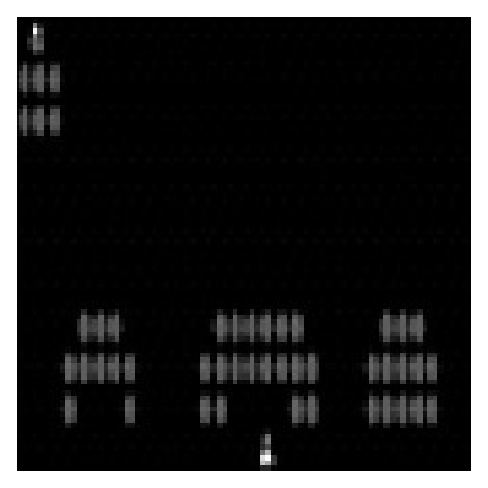
\includegraphics[width=0.3\textwidth]{./fig/alienspp}
    \label{subfig:alienspp}
  } 
  \subfigure[\textit{Boulder Dash}]
  {
    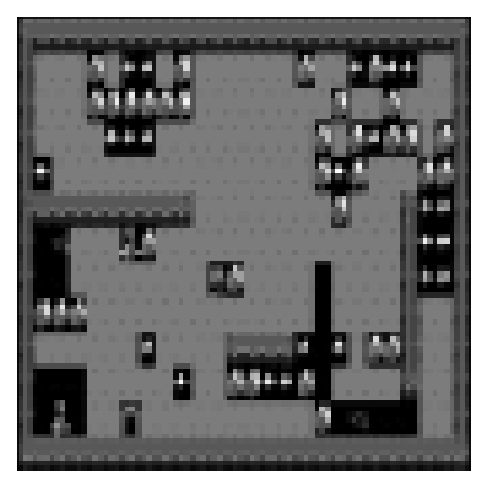
\includegraphics[width=0.3\textwidth]{./fig/boulderdashpp}
    \label{subfig:boudlerdashpp}
  }
  \subfigure[\textit{Missile Commands}]
  {
    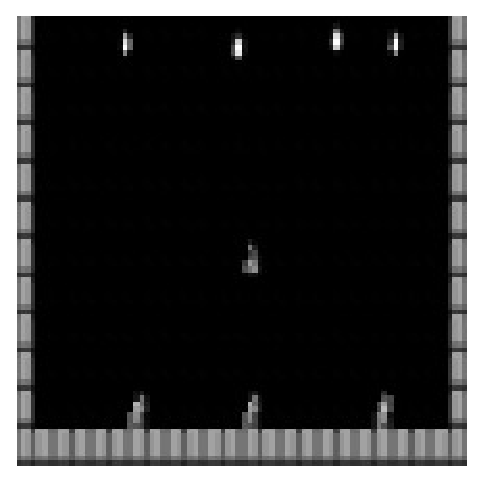
\includegraphics[width=0.3\textwidth]{./fig/missilecommandpp}
    \label{subfig:missilecommandpp}
  }
  \caption{Resultado do pré-processamento das imagens.}
  \label{fig:jogosanalisepp}
\end{figure}

% As imagens pré-processadas são então passadas para o algoritmo \textit{Proximal Policy Optimization} (Seção \ref{section:ppoalg}), que avalia o estado e escolhe uma ação a ser executada. A ação escolhida é passada para o ambiente do GVGAI\_GYM, que então executa a ação no jogo, calcula a recompensa obtida, e retorna o próximo estado. Todo esse processo é repetido até um estado terminal é atingido, indicando que o agente ganhou ou perdeu o jogo, e então o ambiente é reiniciado e o processo começa novamente. para o algoritmo \textit{Proximal Policy Optimization} (Seção \ref{section:ppoalg})

As imagens pré-processadas alimentam duas redes neurais, uma chamada de Ator e outra chamada de Crítico. O modelo Ator é responsável pelo aprendizado de qual ação selecionar a partir de um estado observado do ambiente. Aqui, as imagens do jogo, já pré-processadas, são passadas para uma Rede Neural Convolucional (CNN do inglês \textit{Convolutional Neural Network}) \cite{Krizhevsky12}, que gera como saída uma ação, como andar ou atirar. 

\begin{figure}[ht]
 \centering
  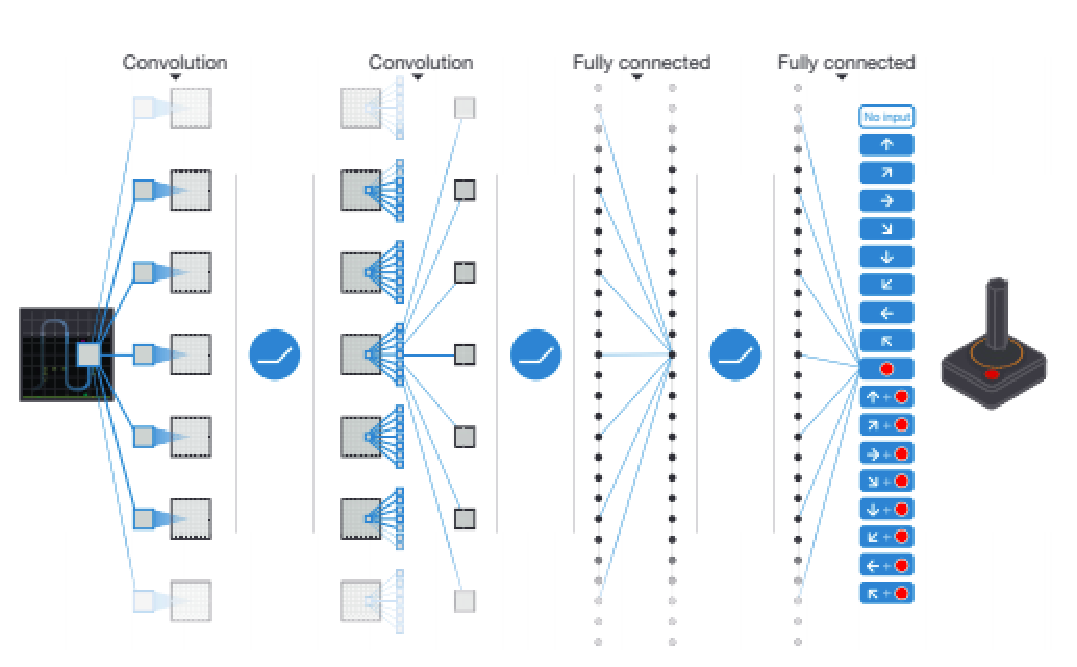
\includegraphics[width=0.8\textwidth]{./fig/cnngame}
  \captionsetup{width=1\textwidth}
 \caption{Ilustração esquemática de uma rede neural convolucional \cite{mnih15}.}
 \label{fig:cnn}
\end{figure}

As ações preditas pelo Ator são passadas para o ambiente do GVGAI\_GYM, que é responsável pela execução da ação no jogo. A ação executada gera uma recompensa que é calculada e retornada juntamente com o próximo estado do jogo. O modelo Crítico deve aprender a avaliar o estado atual, calculando o quão bom o estado é com base em sua recompensa através da função de valor (Função \ref{eqn:value}). Todo esse processo é repetido por uma quantidade finita de passos, em um processo de coleta de trajetórias. Ao final da coleta de trajetórias o valor da função de vantagem (Função \ref{eqn:gae}) é calculado, e os parâmetros do Ator e do Crítico são otimizados com base no Algoritmo \ref{alg:ppoclip}, \textit{Proximal Policy Optimization}. O fluxo de treinamento Ator-Crítico é mostrado na Figura \ref{fig:ac}. As configuração de hiperparâmetros do algoritmo utilizado nos experimentos pode ser conferida no Apêndice \ref{apend:1}, e a implementação do algoritmo pode ser encontrada no Github\footnote{\url{https://github.com/luanagbmartins/general-game-playing}}.

\begin{figure}[ht]
 \centering
  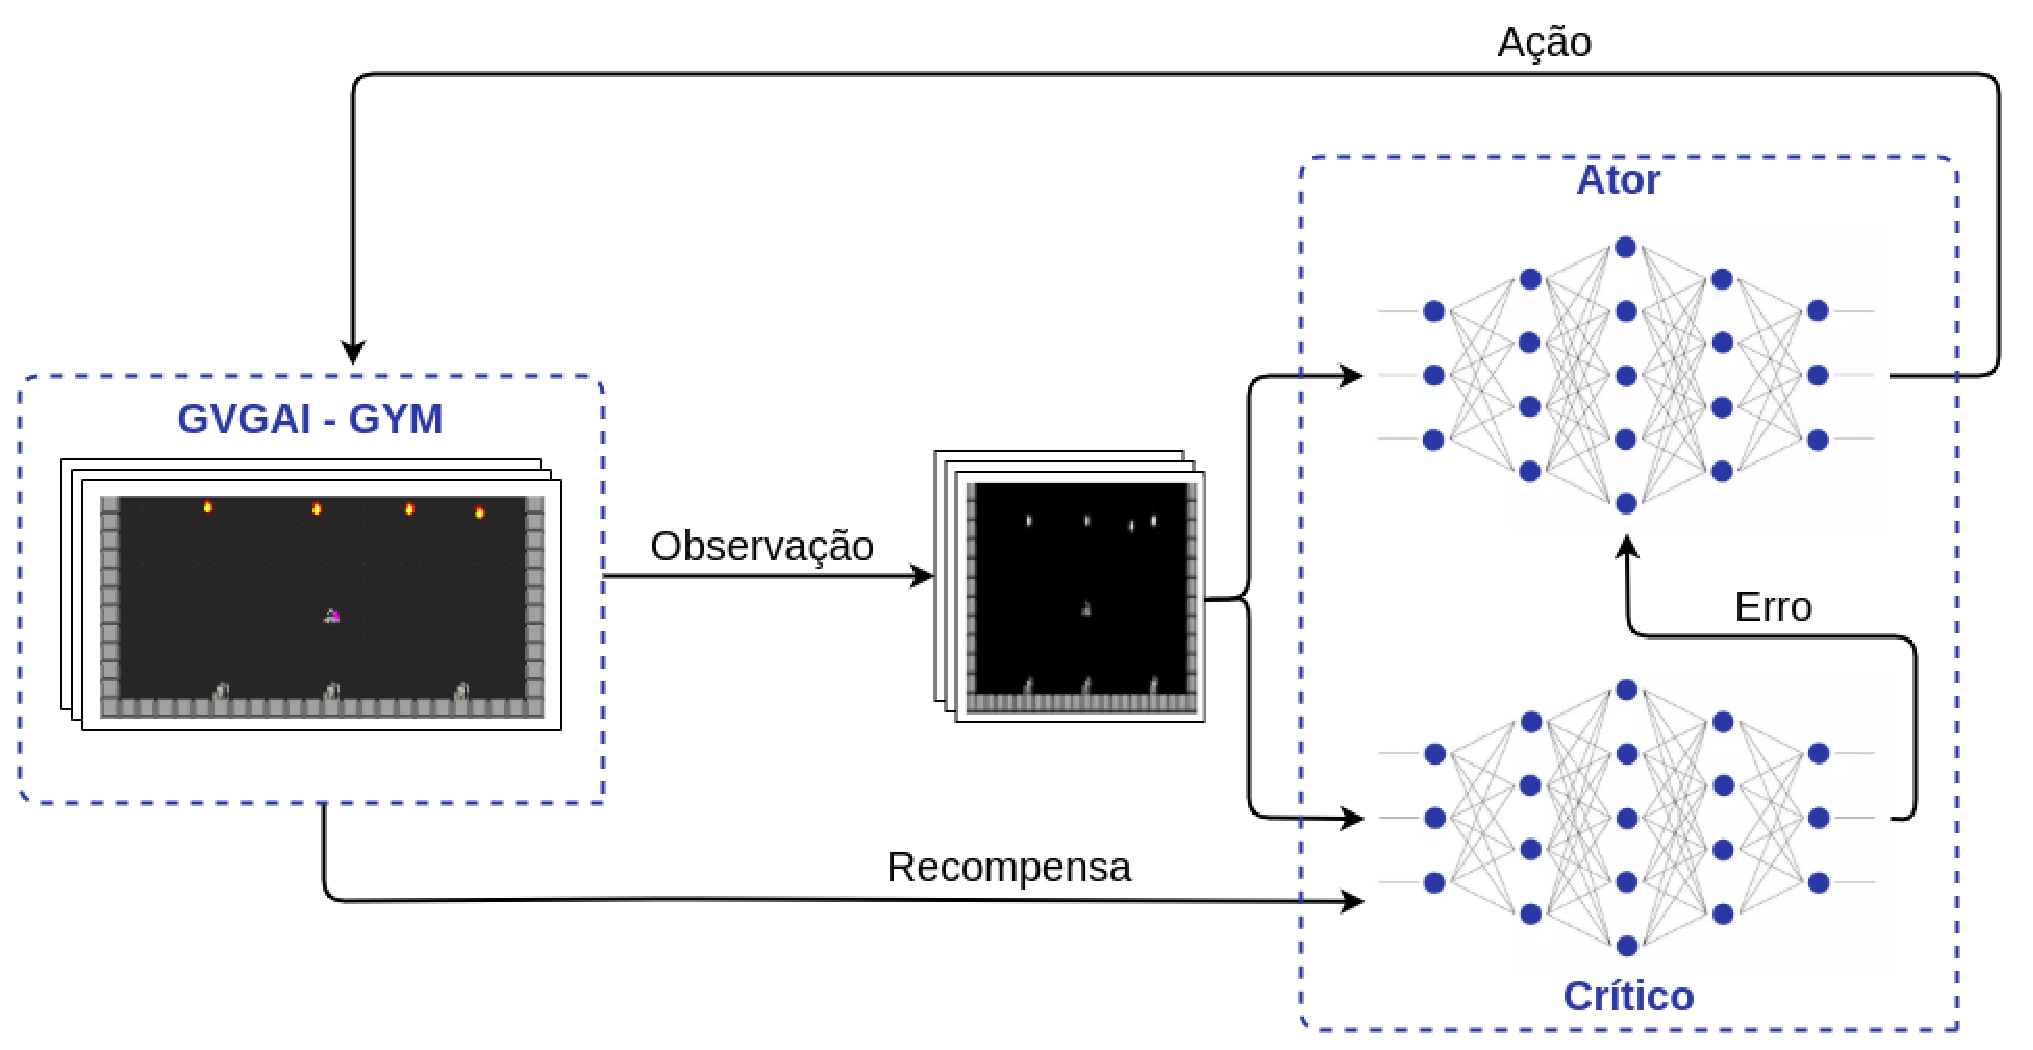
\includegraphics[width=0.92\textwidth]{./fig/ator-critico}
 \caption{Fluxo de treinamento Ator-Crítico.}
 \label{fig:ac}
\end{figure}

% - - - - - - - - - - - - - - - - - - - - - - - - - - - - - - - - - - -
\section{Testes}

Todos os três jogos apresentados na seção anterior são divididos em cinco fases, ou níveis, que serão por sua vez divididos entre conjuntos de treino e teste. Todos os níveis de cada jogo são obtidos da mesma distribuição, portanto a diferença entre o desempenho do conjunto de treinamento e de teste determina o quão super ajustado o agente ficou ao conjunto de treinamento. A medida que o número de níveis de treinamento disponíveis aumenta, espera-se que o desempenho no conjunto de testes melhore, mesmo quando os agentes são treinados para um número fixo de iterações. Para todos os jogos, o treinamento foi limitado a 3 milhões de iterações distribuídas paralelamente entre 8 processos. Cada processo foi responsável por um ambiente do conjunto de treinamento. Os testes de cada jogo foram divididos entre conjuntos de treinamento com uma, duas e três fases. As fases não utilizadas em treinamento irão compor o conjunto de testes utilizados na fase de avaliação do agente.

\chapter{Resultados}
\label{cap:resultados}

Neste capítulo serão apresentados e analisados todos os resultados obtidos do treinamento do \textit{Proximal Policy Optimization} (PPO) para jogar os jogos disponibilizados pela ferramenta GVGAI\_GYM, \textit{Aliens}, \textit{Boulder Dash} e \textit{Missile Command}. Os jogos selecionados variam em termos de recompensas que eles oferecem, e as recompensas disponíveis possuem um grande impacto no sucesso do aprendizado por reforço. Para cada um dos jogos, foi modificado o tamanho do conjunto de treinamento, ou seja, a quantidade de fases disponíveis para treinamento, sendo divididos em conjuntos com um nível de treinamento (PPO1), dois níveis de treinamento (PPO2) e três níveis de treinamento (PPO3). 

Cada fase de um jogo difere em sua dificuldade, definindo o quão desafiante é o jogo. O nível de dificuldade varia na adição ou remoção de eventos desafiadores ou obstáculos para alcançar o objetivo final. A medida que um jogador avança nas fases disponíveis, ele esbarra em desafios cada vez mais complexos, exigindo mais planejamento estratégico e reações rápidas para ser capaz de lidar com as adversidades.

Durante o treinamento do agente uma política é selecionada para interagir com o ambiente em um número fixo de etapas, com o objetivo de coletar um conjunto de experiências. Essas experiências são então utilizadas para atualizar o modelo. Para cada lote de experiências é calculado uma média das recompensas totais dos últimos dez episódios concluídos. A cada dez atualizações do modelo o agente é submetido a uma avaliação de desempenho nos ambientes de testes. A Figura \ref{fig:resultados} contém as informações suavizadas\footnote{O filtro de Savitzky-Golay pela biblioteca Scipy foi utilizado como uma janela de tamanho 53 e ordem polinomial 3.} de média das recompensa obtidas pelo agente durante o treinamento (cores mais escuras) e uma média das recompensas de dez episódios da fase de avaliação (cores mais claras). 

A medida que o número de interações com o ambiente aumenta é esperado que as recompensas durante o treinamento também aumentem: cada atualização deve levar a políticas que maximizem cada vez mais a recompensa obtida. Se o treinamento chegar a tal ponto em que a cada atualização não é observado uma mudança significativa dos valores de retorno, como visto na Figura \ref{subfig:missilecommand-r} para o PPO1,então diz-se que foi atingido um máximo local do problema de otimização da política. 

\begin{table}[H]
\centering
 \begin{tabular}{||c c c c c c c ||} 
 \hline
 Jogos & Agente Aleatório & PPO 1 & PPO 2 & PPO 3 & DQN & A2C\\ [0.5ex] 
 \hline\hline
 Aliens & 38 & 62.7 & 62.7 & 63.5 & 75 & \textbf{77}\\ [1ex] 
 \hline
 Boulder Dash &  1.69 & 19.8 & 19.8 & \textbf{20} & 2.5 & 15.5\\ [1ex] 
 \hline
 Missile Command & -1.46 & 5 & \textbf{11.6} & 10.3 & 5 & 5\\ [1ex] 
 \hline
\end{tabular}
\caption{Comparação das recompensas obtidas para cada jogo.}
\label{tab:allgames}
\end{table}

Na Tabela \ref{tab:allgames} é possível comparar os melhores resultados de treinamento de cada jogo com os melhores resultados dos algoritmos de aprendizado por reforço \textit{Deep Q-Network} (DQN) \cite{mnih13} e \textit{Advantage Actor Critic} (A2C) \cite{openaibaselines} obtidos de Torrado et.tal. \cite{torrado18}, e de um agente com política aleatória. Em ambos \textit{Boulder Dash} e \textit{Missile Command} o algoritmo PPO se sobressaiu aos demais, obtendo pior desempenho apenas no jogo \textit{Aliens}.

Apesar de não ter ultrapassado os outros algoritmos de aprendizado por reforço (Tabela \ref{tab:allgames}), o agente no jogo \textit{Aliens} conseguiu aprender a jogar o jogo razoavelmente bem no conjunto de treinamento. Todos os personagens não-jogáveis e projéteis deste jogo se comportam de maneira determinística e o jogo pode ser jogado bem com muito pouco planejamento, o que pode levar o agente a explorar brechas de posicionamento dos jogos de treinamento. Uma vez que o cenário sofre mudanças entre as fases, o pouco planejamento pode resultar em um superajustamento do conjunto de treinamento. Apesar dos agentes aprenderem a jogar o jogo de maneira satisfatória, falham em conseguir generalizar seu objetivo, não conseguindo obter desempenho satisfatório no conjunto de teste, como pode ser observado na Figura \ref{subfig:aliens-r}. 

\begin{figure}[ht]
 \begin{center}
  \subfigure
  {
    \includegraphics[width=0.48\textwidth]{./fig/gvgai-aliens-lvl0-v0-frame94}
    \label{subfig:a-frame1}
  } 
  \subfigure
  {
    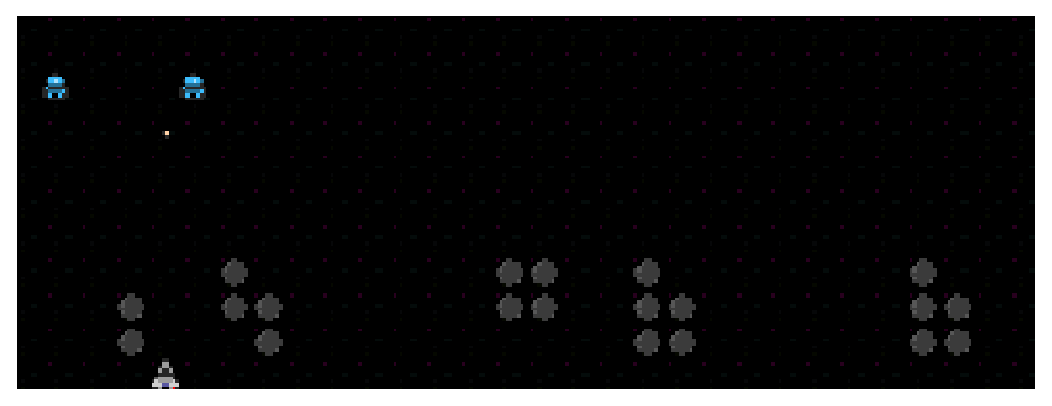
\includegraphics[width=0.48\textwidth]{./fig/gvgai-aliens-lvl0-v0-frame95}
    \label{subfig:a-frame2}
  }
  \caption{Exemplos de execução do jogo \textit{Aliens}.}
  \label{fig:aliensframe}
\end{center}
\end{figure}

No \textit{Boulder Dash}, quando o jogador coleta um diamante por pontos, uma pedra pode cair em sua na direção. Isso significa que existe um retorno negativo se um agente coleta um diamante e não se mover. Não coletar nenhum diamante e sobreviver parece uma ótima solução local de que os agentes têm dificuldade em escapar. Entretanto, todos os três agentes conseguiram boas pontuações durante o treinamento (Tabela \ref{tab:allgames}), indicando sucesso em conseguir contornar essa dificuldade. Apesar de conseguir aprender bem essa mecânica do jogo, observando a Figura \ref{subfig:boulderdash-r} o agente falha em conseguir abstrair o objetivo geral, ficando limitado no aprendizado de um conjunto de ações específicas para o ambiente em que foi treinado. 

\begin{figure}[ht]
 \begin{center}
  \subfigure
  {
    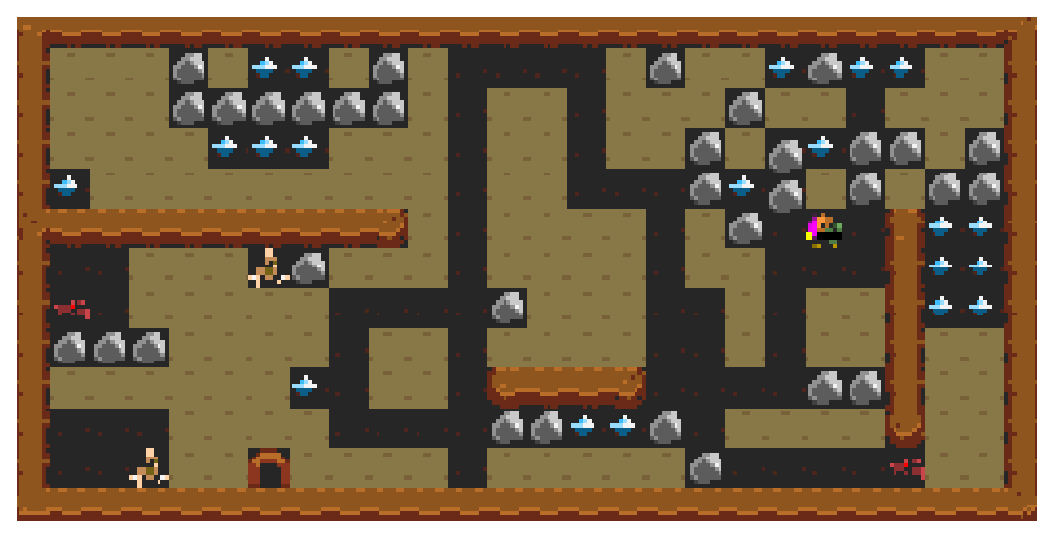
\includegraphics[width=0.48\textwidth]{./fig/gvgai-boulderdash-lvl0-v0-frame25}
    \label{subfig:b-frame1}
  } 
  \subfigure
  {
    \includegraphics[width=0.48\textwidth]{./fig/gvgai-boulderdash-lvl0-v0-frame26}
    \label{subfig:b-frame2}
  }
  \caption{Exemplos de execução do jogo \textit{Boulder Dash}.}
  \label{fig:boulderdashframe}
\end{center}
\end{figure}

Por fim, o \textit{Missile Command} parece ser possível de se jogar simplesmente aproximando-se dos mísseis mais próximos e os atacando. Entretanto é necessário um tempo de reação hábil para conseguir defender todos os canhões a tempo. As recompensas totais de cada fase variam conforme o número de canhões e mísseis inimigos também mudam, gerando uma distribuição de recompensas não linear. Na primeira fase do jogo, por exemplo, há quatro bolas de fogo e três canhões, levando a um total de oito pontos de recompensa. No PPO1 o agente não parecia ser capaz de manter uma pontuação perfeita pois alguns erros levaram a cinco pontos. Entretanto, em ambos PPO2 e PPO3 (Tabela \ref{tab:allgames}), os agentes foram capazes de melhorar sua performance, atingindo pontuação máxima na primeira fase do jogo. Apesar da variedade de exemplos no conjunto de treinamento ter levado a uma melhor exploração do conjunto de ação-estado, assim como nos outros jogos, é possível observar na Figura \ref{subfig:missilecommand-r} que os agentes ficaram restritos a um conjunto de sequência de ações que levaram ao sucesso nos jogos de treinamento.

\begin{figure}[ht]
 \begin{center}
  \subfigure
  {
    \includegraphics[width=0.48\textwidth]{./fig/gvgai-missilecommand-lvl0-v0-frame12}
    \label{subfig:m-frame1}
  } 
  \subfigure
  {
    \includegraphics[width=0.48\textwidth]{./fig/gvgai-missilecommand-lvl0-v0-frame13}
    \label{subfig:m-frame2}
  }
  \caption{Exemplos de execução do jogo \textit{Missile Command}.}
  \label{fig:missilecommandframe}
\end{center}
\end{figure}

Na Figura \ref{fig:avaliacao} é possível observar o desempenho médio de cada agente treinado, ao longo das cinco fases dos três jogos, em comparação a um agente com política aleatória. Assim como no jogo \textit{Missile Command}, todos os agentes foram direcionados a uma melhor exploração do espaço de ações a medida que aumentava a variedade da amostragem do conjunto de treinamento, levando a um aumento de desempenho geral ao longo das cinco fases de cada jogo. No entanto, nas fases que não foram utilizadas para compor o conjunto de treinamento, o desempenho se manteve muito próximo do agente com política aleatória.

% \begin{figure}[ht]
%  \centering
%   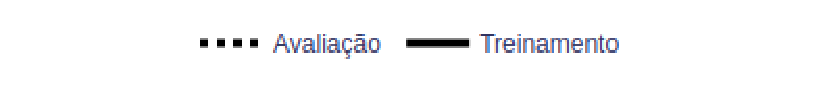
\includegraphics[width=0.3\textwidth]{./fig/legend}
% \end{figure}

\begin{figure}[hb]
 \begin{center}
 \subfigure
  {
    \centering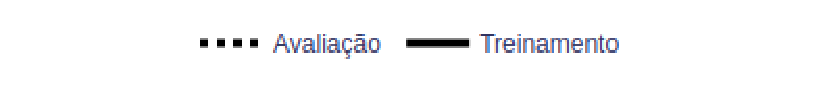
\includegraphics[width=0.49\textwidth]{./fig/legend}
  } 
  \subfigure[\textit{Aliens}]
  {
    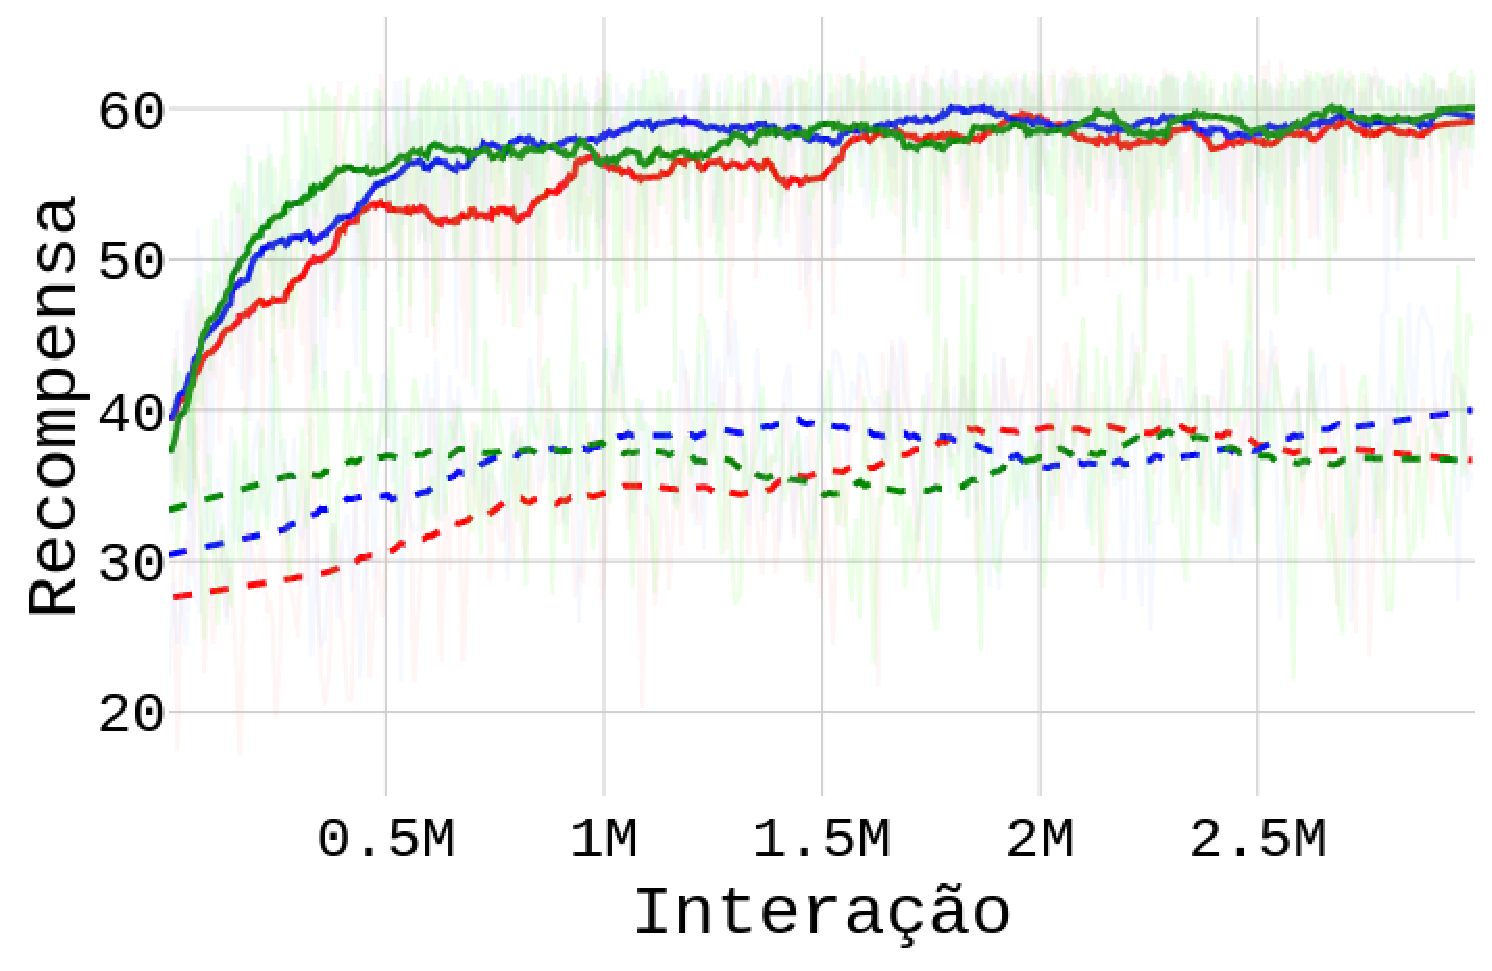
\includegraphics[width=0.48\textwidth]{./fig/aliens-results}
    \label{subfig:aliens-r}
  } 
  \subfigure[\textit{Boulder Dash}]
  {
    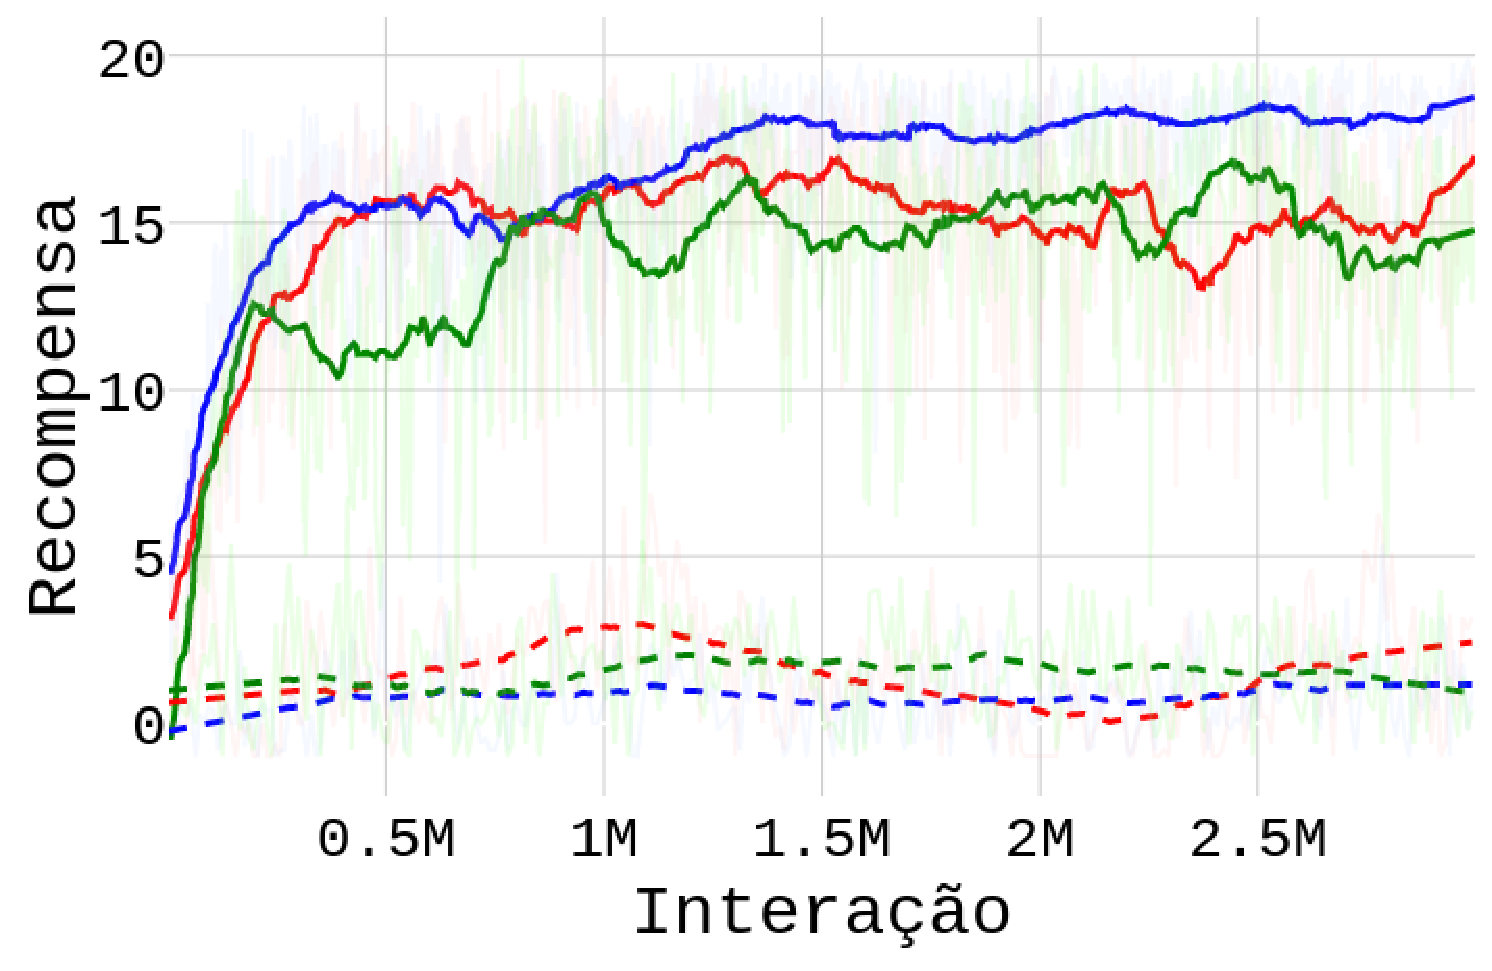
\includegraphics[width=0.48\textwidth]{./fig/boulderdash-results}
    \label{subfig:boulderdash-r}
  }
  \subfigure[\textit{Missile Command}]
  {
    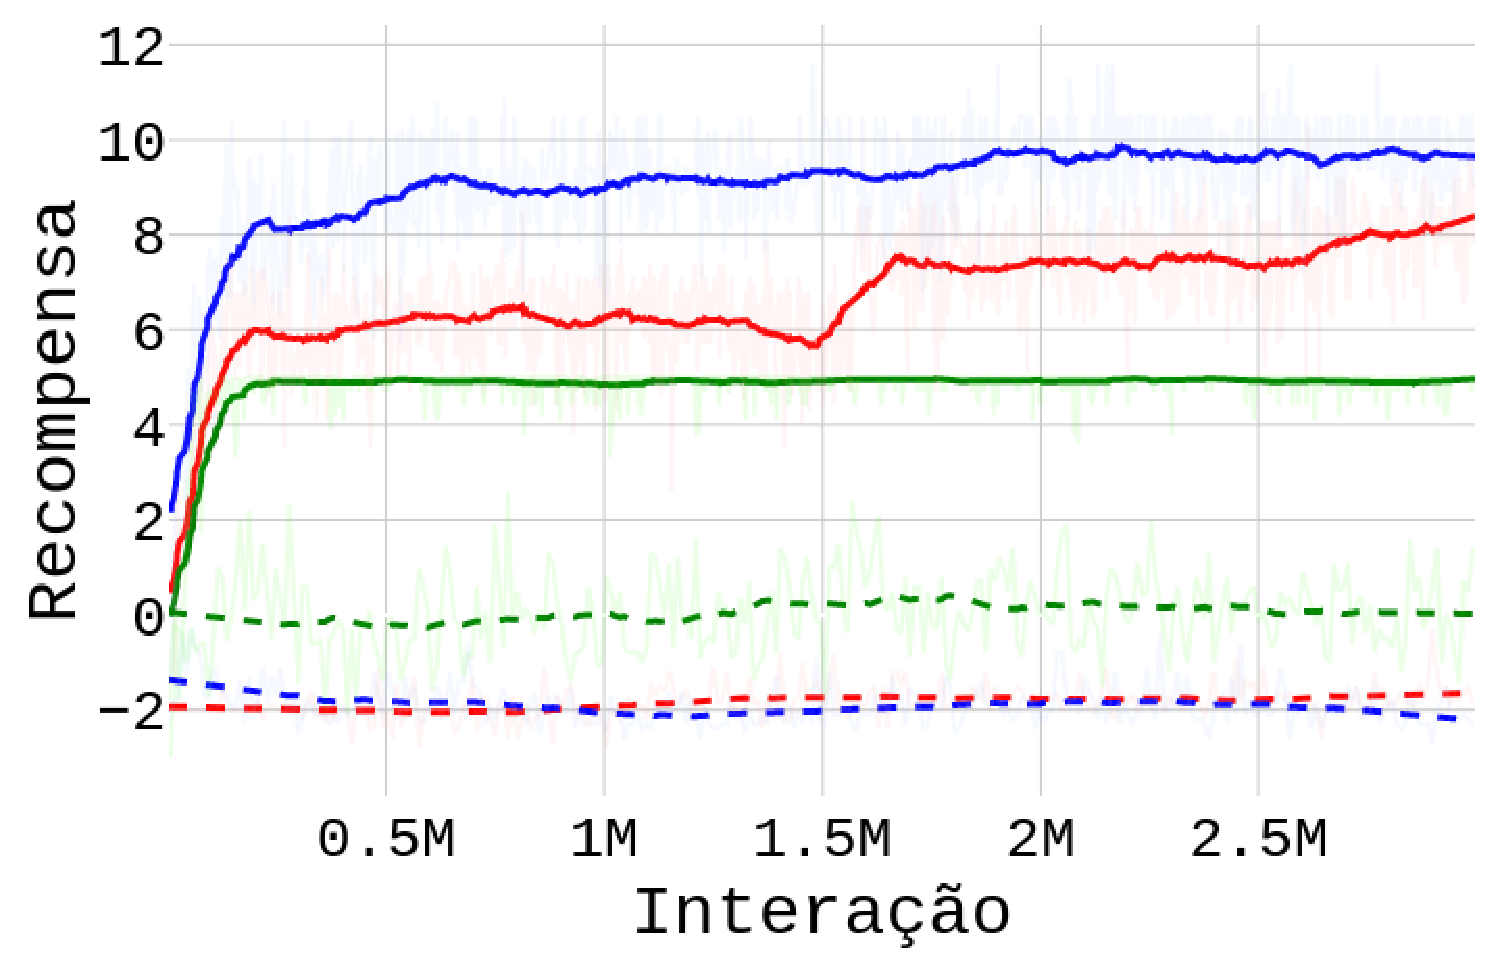
\includegraphics[width=0.48\textwidth]{./fig/missilecommand-results}
    \label{subfig:missilecommand-r}
  }
  \captionsetup{width=1\textwidth}
  \caption[Gráfico de relação treinamento-avaliação.]
  {Gráfico de relação treinamento-avaliação. Em vermelho, conjunto de treinamento com três fases (PPO3); em azul, conjunto de treinamento com duas fases (PPO2); em verde, conjunto de treinamento com uma fase (PPO1).}
  \label{fig:resultados}
\end{center}
\end{figure}
\begin{figure}[ht]
  \centering
  \subfigure[\textit{Aliens}]
  {
    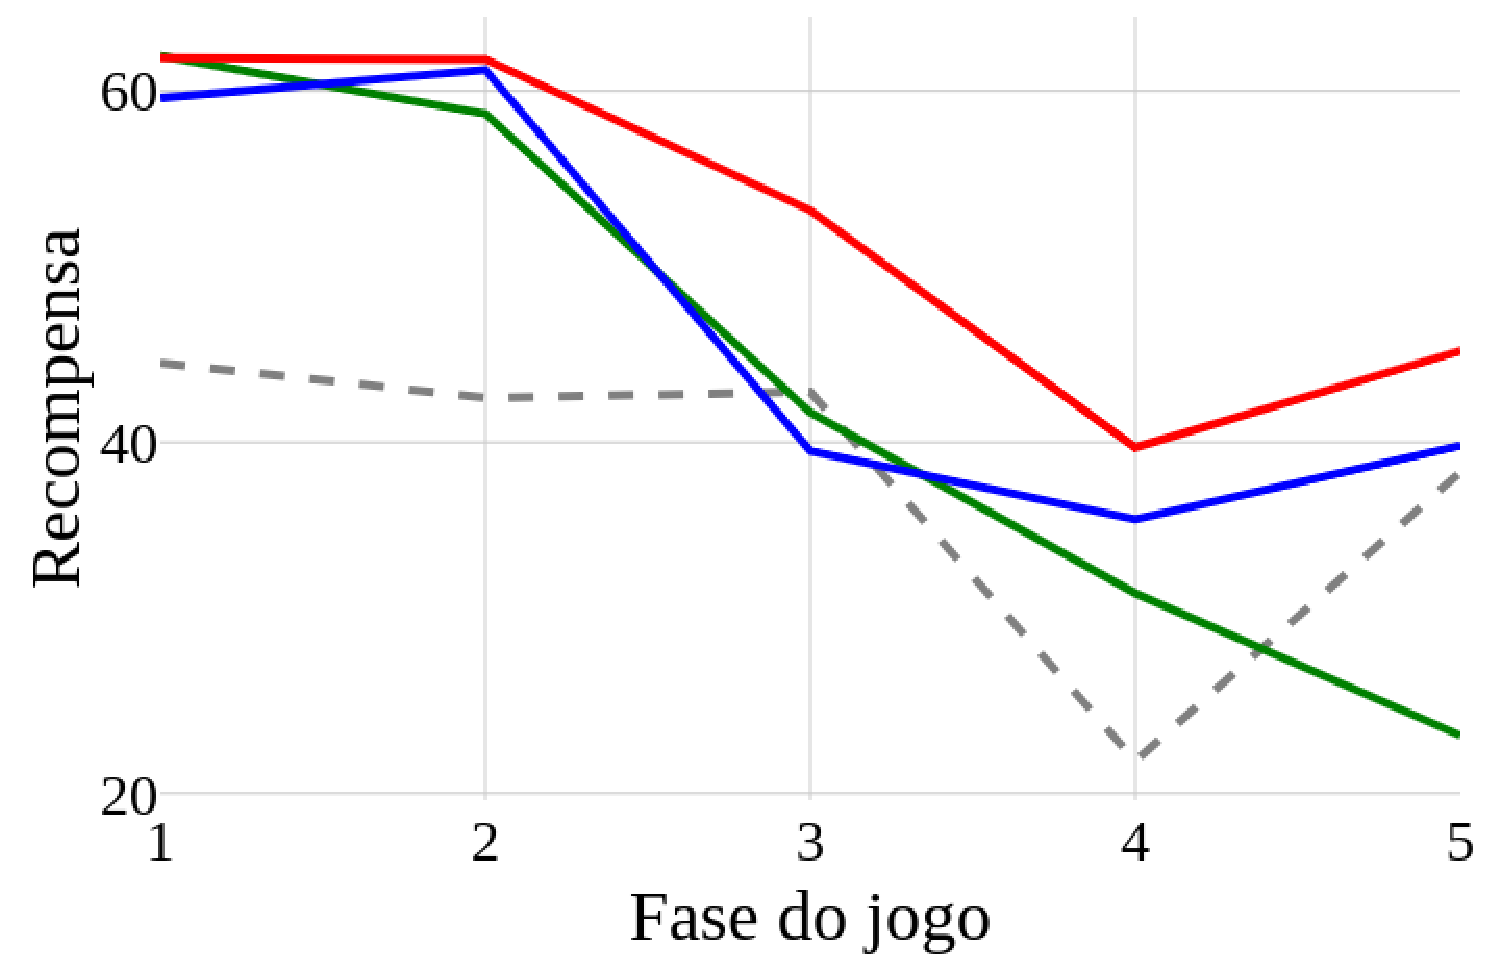
\includegraphics[width=0.45\textwidth]{./fig/aliens-evaluation}
    \label{subfig:aliens-a}
  } 
  \subfigure[\textit{Boulder Dash}]
  {
    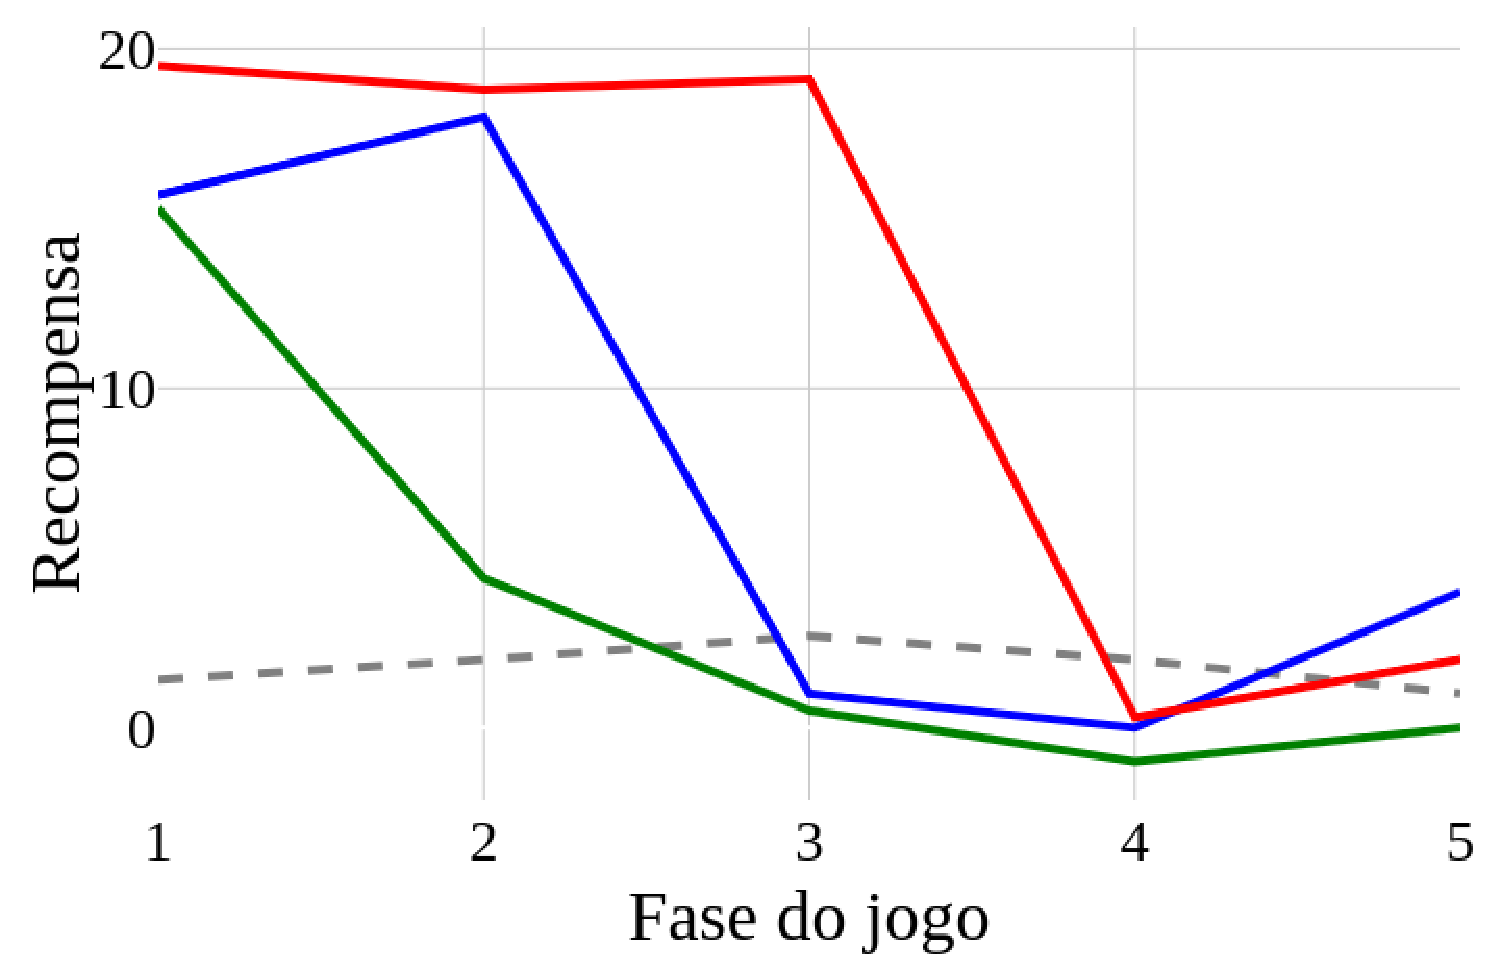
\includegraphics[width=0.45\textwidth]{./fig/boulderdash-evaluation}
    \label{subfig:boulderdash-a}
  }
  \subfigure[\textit{Missile Command}]
  {
    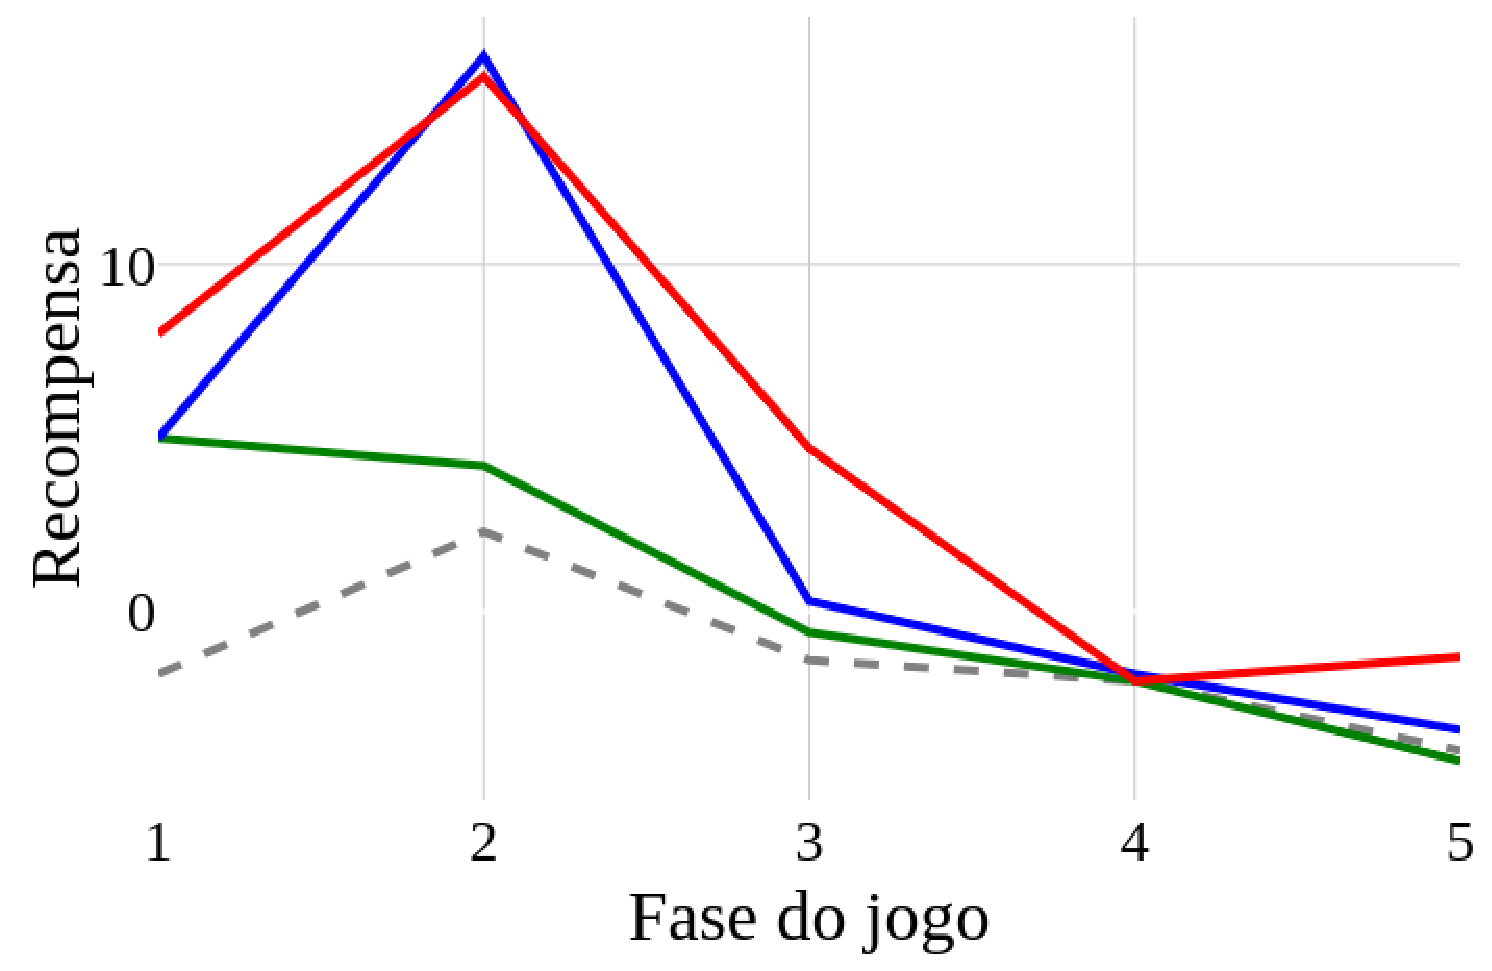
\includegraphics[width=0.45\textwidth]{./fig/missilecommand-evaluation}
    \label{subfig:missilecommand-a}
  }
  \captionsetup{width=1\textwidth}
  \caption[Gráfico de recompensa dos modelos treinados.]
  {Gráfico de recompensa dos modelos treinados. Em vermelho, conjunto de treinamento com três fases (PPO3); em azul, conjunto de treinamento com duas fases (PPO2); em verde, conjunto de treinamento com uma fase (PPO1); em linhas tracejadas, agente com política aleatória. }
  \label{fig:avaliacao}
\end{figure}
\chapter{Conclusão}
\label{cap:conclusao}

Neste trabalho foram estudados os conceitos de aprendizado de máquina, em especial o aprendizado por reforço. Dentre as diferentes técnicas que podem ser utilizadas para realizar a tarefa de aprendizado por reforço, as abordagens baseadas em redes neurais profundas têm apresentado resultados satisfatórios no aprendizado de problemas complexos de alta dimensão. Dentre essas técnicas, destaca-se o algoritmo \textit{Proximal Policy Optimization} (PPO), que obteve melhor desempenho geral em comparação a outros algoritmos de aprendizado por reforço.

Apesar dos grandes avanços realizados durante os últimos anos no desenvolvimento de algoritmos que aprendem tipos específicos de problemas, os agentes falham em generalizar entre tarefas, o que se mostrou não ser diferente para o algoritmo PPO. Contudo, os ambientes de avaliação de aprendizado por reforço insistem em avaliar o desempenho dos algoritmos nos mesmos ambientes de treinamento. Quando é divulgado que um algoritmo foi capaz de aprender uma política capaz de jogar bem um jogo, pode significar, na verdade, que a política encontrou ações ideais para o espaço de observações que o jogo fornece. 


Nos testes realizados foram observados que os agentes tendem a explorar o determinismo do ambiente, ignorando os estados e memorizando sequências de ação efetivas que os levam a atingir pontuações cada vez maiores, sem aprender conceitos gerais do jogo. Esses agentes sofrem de sobre-ajuste ao conjunto de treinamento, sendo sensíveis a pequenas perturbações nos ambientes e incapazes de generalizar para estados não vistos anteriormente. Entretanto, foi possível notar que conjuntos de treinamento com uma maior variedade contribuem para uma melhor exploração da política, levando a resultados melhores em comparação a conjuntos de treinamento com baixa variedade. Acredita-se que esse aumento no desempenho do treinamento provém de um currículo implícito fornecido por um conjunto diversificado de fases. 

Em um ambiente de aprendizado supervisionado, a generalização é obtida treinando um modelo em um grande conjunto de dados, geralmente com milhares de exemplos. A introdução de fases geradas proceduralmente, encorajadas pelo GVGAI\_GYM, permite que os comportamentos treinados generalizem para fases não vistas na distribuição do treinamento. Entretanto, os agentes sofrem para generalizar a partir de poucas fases de treinamento disponíveis.

De maneira equivalente ao aprendizado supervisionado, os algoritmos de aprendizado por reforço devem alcançar uma boa generalização se muitas variações dos ambientes forem usadas durante o treinamento. Trabalhos recentes exploram essa preocupação gerando proceduralmente enormes conjuntos de treinamento e teste para avaliar melhor a capacidade de generalização dos algoritmos \cite{cobbe2019, cobe18}, reforçando que algoritmos de aprendizado por reforço ainda são ineficientes em termos de amostragem.

Como trabalhos futuros são propostas algumas direções com foco em uma melhor eficiência de amostragem, buscando diminuir a necessidade de grandes conjuntos de treinamento. Maiores investigações devem ser realizadas do impacto de diferentes arquiteturas e formas de regularização, como sugerido em \cite{cobe18}. Além disso, \cite{curiositylarge, pathak} fazem uso de modelos de dinâmica inversa afim de melhorar a extração de características da observação, de forma que características mais importantes para a decisão do agente tenham uma maior importância. Isso pode ser explorado no contexto de generalização por poder desencorajar a memorização de sequência de ações efetivas. 



% Por fim, essas ideias podem ser aplicadas no contexto de robótica para diminuir a dificuldade de levar um modelo treinado em um ambiente de simulação para a vida real.


% Além disso, pesquisas mostram que os agentes de aprendizado por reforço orientados pela curiosidade foram capazes de generalizar melhor com ambientes inexplorados .


% Ainda que o aprendizado por reforço tem se mostrado muito bem-sucedido em ambientes fechados, como jogos eletrônicos, é difícil de ser aplicado em ambientes do mundo real. Como visto neste trabalho, o aprendizado por reforço é ineficiente em termos de amostragem, exigindo uma vasta quantidade de exemplos de treinamento para aprender tarefas mais complexas. Para aplicações no mundo real, a ausência da capacidade de generalização abre grandes lacunas entre ambientes simulados e reais que dificultam o treinamento de modelos.  

% Como trabalhos futuros são propostas algumas direções com o objetivo de melhorar o aprendizado de agentes inteligentes, com foco em uma melhor eficiência de amostragem. Maiores investigações devem ser realizadas do impacto de diferentes arquiteturas e formas de regularização, como realizado em \cite{cobe18}. Além disso, pesquisas mostram que os agentes de aprendizado por reforço orientados pela curiosidade foram capazes de generalizar melhor com ambientes inexplorados \cite{curiositylarge, pathak}.

% No geral, encontramos algumas evidências promissoras que mostram que as habilidades aprendidas pela curiosidade ajudam nosso agente a explorar com eficiência em novos ambientes.

% Por outro lado, a adaptação ao meio de interação nem sempre são indesejáveis. Seres humanos constantemente super-ajustam sub-rotinas através de memórias musculares, permitindo agir de maneira hábil eficientemente na maioria das situações do dia-a-dia. Contudo, uma das principais habilidades dos seres humanos é sua capacidade em detectar falhas provenientes dessas ações automáticas e se adaptar, sendo capaz de lidar com as adversidades.

% Para que os agentes de aprendizagem por reforço possam ser confiáveis para atuar em situações de alto risco no mundo real, é necessário o desenvolvimento da capacidade de lidar com falhas e situações inesperadas. É necessário portanto generalizar sobre os perigos comuns que poderia ter sido experimentado antes, mas em um ambiente não visto anteriormente, para então pode ser implanto com segurança no mundo real.


%------------------------------------------------------------ BIBLIOGRAFIA %
\cleardoublepage
\arial
\bibliography{modelo-tese} %%% Nomes dos seus arquivos .bib
\label{ref-bib}

%--------------------------------------------------------------- APÊNDICES %
\apendices

\chapter{Hiperparâmetros}
\label{apend:1}

\begin{table*}[ht]
\centering
\caption{Hiperparâmetros para o algoritmo PPO.}
\label{tab:hiperparameters} 
\begin{tabular}{|c|c|}
\hline Hiperparâmetro & Valor \\
\hline Iterações (total) & $3x10^5$ \\
\hline Taxa de aprendizado & $2.5^{-4}$ \\
\hline Coeficiente de entropia & $0.01$ \\ 
\hline Parâmetro $\epsilon$ de corte (PPO) & $0.2$ \\
\hline Tamanho do episódio & $128$ \\ 
\hline Tamanho do lote & $32$ \\ 
\hline $\gamma$ & $0.99$ \\ 
\hline $\lambda$ & $0.95$ \\ 
\hline 
\end{tabular} 
\end{table*}
% \input{./pos/apend_II}

\end{document}

%------------------------------------------------------------------------- %
%        F I M   D O  A R Q U I V O :  m o d e l o - t e s e . t e x       %
%------------------------------------------------------------------------- %
